%\documentclass[11pt,a4paper]{article}
%\documentclass[11pt,a4paper]{scrartcl}
\documentclass[11pt,a4paper,oneside]{book}
\usepackage[british,UKenglish,USenglish,english,american]{babel}
%\usepackage[a4paper, total={16cm, 23cm}]{geometry}
\usepackage[tmargin = 1.25in,bmargin = 1.25in,lmargin = 1in,rmargin = 
1in]{geometry}
\usepackage[table]{xcolor}
\usepackage{tikz}
\usepackage{graphicx}
\usepackage{pgfplots}
\pgfplotsset{width=12cm,compat=1.9}
\usepackage{setspace}
\usepackage{chemmacros}
\usepackage{chemfig}
%\usepackage{ghsystem}
%\usechemmodule{redox}
%\usepackage{chemnum}
%\usepackage{bohr}
%\usepackage{elements}
%\usepackage{endiagram}
%\usepackage{modiagram}
%\usepackage{chemgreek}
%\usepackage{mhchem}
\usepackage{esint}
\usepackage{tabularray}

\usepackage{makeidx}
\usepackage{epstopdf}

\usepackage{amssymb}
\usepackage{mathrsfs}
%\usepackage{minted}
\usepackage{bm}
\usepackage{amsmath}
\usepackage{enumitem}
\usepackage[english]{varioref}
\usepackage[english]{babel}
\usepackage{lipsum}
\usepackage{fancyhdr}
\pagestyle{fancy} 
\usepackage{float}
\usepackage{empheq}
\usepackage[framemethod=tikz]{mdframed}
\usepackage{epstopdf}
\numberwithin{equation}{section}
\usepackage{eso-pic}
\usepackage{calc}
\usepackage{nccmath}
\usepackage{caption}
\usepackage{subcaption}
\usepackage{gensymb}
\usepackage{amsfonts,amsthm,epsfig,epstopdf,titling,url,array}
\usepackage{siunitx}
\sisetup{input-digits = 0123456789\pi}
\usepackage[symbol]{footmisc}
\usepackage{xcolor}
\usepackage{multicol}
\usepackage{longtable}
\usepackage{boondox-cal}
\DeclareSIUnit\atm{atm}
\setcounter{secnumdepth}{3}
\setcounter{tocdepth}{3}
\usepackage{booktabs}
\usepackage{blindtext}
\usepackage{changepage}

% \usepackage{draftwatermark}
% \SetWatermarkText{DRAFT}
% \SetWatermarkScale{5}

\DeclareSIUnit\atm{atm}

\pagestyle{fancy} 
\fancypagestyle{firstpage}{
\rhead{
%	\begin{picture}(0,0) 
%			\put(-30,0){
\includegraphics[width=1cm]{figures/MCI_4C_bw.eps}} 
%	\end{picture}
}
}
\fancyhead[L]{\slshape\nouppercase{\leftmark}}
\chead{}
\rhead{
%	\begin{picture}(0,0) 
%		\put(-30,0){
\includegraphics[width=1cm]{figures/MCI_4C_bw.eps}} 
%	\end{picture}
}
\lfoot{\textit{}}
\cfoot{-\ \thepage\ -}
\rfoot{\textit{}}

\DeclareMathOperator{\rank}{rank}
\DeclareMathOperator{\atantwo}{atan2}
\DeclareMathOperator{\spn}{span}

\renewcommand{\headrulewidth}{0.4pt}
\renewcommand{\footrulewidth}{0.4pt}
\newcommand{\abs}[1]{\left|#1\right|}
\definecolor{mycolor1}{rgb}{0.97, 0.97, 0.97}
\definecolor{mycolor2}{rgb}{0.97, 0.97, 0.97}
\definecolor{tableShade}{gray}{0.9}
\newcommand{\sign}{\text{sign}}
\newcommand{\centered}[1]{\begin{tabular}{@{}l@{}} #1 \end{tabular}}
\theoremstyle{it}
\newtheorem{defn}{Definition}[chapter]
\newtheorem{assumption}{Assumption}[chapter]
\newtheorem{thm}{Theorem}[chapter]
\newtheorem{lemma}{Lemma}[chapter]
\newtheorem{corollary}{Corollary}[chapter]
%\newtheorem{defn}{Definition}[section]
%\newtheorem{assumption}{Assumption}[section]
%\newtheorem{thm}{Theorem}[section]
%\newtheorem{lemma}{Lemma}[section]
%\newtheorem{corollary}{Corollary}[section]
\theoremstyle{definition}
%\theoremstyle{it}
\newtheorem{example}{Example}[section]

\newenvironment{myitemize_1}
{ \begin{itemize}[topsep=0pt]
		\setlength{\topsep}{2pt}		
		\setlength{\itemsep}{2pt}
		\setlength{\parskip}{2pt}
		\setlength{\parsep}{2pt}     }
	{ \end{itemize}                  }


\newmdenv[innerlinewidth=0.5pt, roundcorner=4pt,backgroundcolor=mycolor2, 
linecolor=mycolor1,innerleftmargin=6pt,
innerrightmargin=6pt,innertopmargin=6pt,innerbottommargin=6pt]{mybox}

\title{\textbf{ 
	\begin{LARGE}
		Propeller Electrical Power-train Design
	\end{LARGE} \\[24pt]
	\begin{Large}
		Model, control strategy and hardware dimensioning 
	\end{Large}}
}
\author{\textbf{Davide Bagnara}}

\begin{document}
%	\begin{onehalfspace}
	\thispagestyle{firstpage}
	\begin{mybox}
		\maketitle
		\vspace{120mm}
	\end{mybox}
	\newpage
	\tableofcontents
	\listoffigures	
	\listoftables
	\newpage
	

\chapter{Preliminary Electro-thermal Simulations}
The following chapter concerns the preliminary dimensioning of an electrical drive for permanent magnet synchronous motor (PMSM) for drone application. The chapter in question consists of the following parts:
\begin{itemize}
	\item[--] parameters identification of the selected PMSM;
	\item[--] preliminary dimensioning of the hardware components, DClink, MOSFET, Heat-Sink, etc.;
	\item[--] preliminary electro-thermal performance evaluation via Simulink/Simscape modelization;	
	\item[--] thermal analysis.
\end{itemize}

\section{Motor Parameter Identification}
In this section the motor data are here summarized and the main motor parameters, necessary for the Simulink model implementation as well as for the preliminary electrical dimensioning, are here extrapolated. \\

\noindent \textbf{The motor in question is here reported as follows}:
\begin{itemize}
	\item[--] MAD M50C35 EEE 9KV.
\end{itemize} 

The M50C35 EEE 9KV PMSM synchronous motor is supplied by \textit{MAD Components}, and the main characteristics, in term of voltage/current for nominal torque rating are referred to the DC-Battery stage, as Table~\ref{M50C35EEE9KV_table_1} reproduces.

\begin{table}[H]
	%	\footnotesize
	\small
	\begin{center}	
		\begin{tblr}{p{0.5\linewidth}|p{0.5\linewidth}}
			\textbf{Quantity} & \textbf{Nominal value} \\
			\hline
			Motor Model	& M50C35 EEE 9KV \\	
			Nominal DC Voltage (battery side) &	100S (lipo) -- (\SI{360}{\volt} - \SI{400}{\volt}) -- Max \SI{126}{\celsius} \\
			RPM/V	& 9 \\
			\hline
			Internal Battery Resistance  & \SI{59}{\milli\ohm} \\
			Maximum DC Current & \SI{49.1}{\ampere} \\
			Maximum Torque     & \SI{64}{\newton\meter} \\
			Maximum Power      & \SI{19.5}{\kilo\watt} \\
			Nominal RPM        & \SI{2291}{\per\minute} \\	
			Number of poles    &			62 \\
			\hline
			Recommended ESC    & MAD AMPX 60A (100S) \\
			Motor Weight       & \SI{4.2}{\kilogram} \\
			\hline
		\end{tblr}
	\end{center}
	\captionsetup{width=.5\textwidth, font=small}
	\caption{Motor Parameters from MAD Components Specification.}
	\label{M50C35EEE9KV_table_1}
\end{table}	

\begin{table}[H]
	%	\footnotesize
	\small
	\begin{center}	
		\begin{tblr}{p{0.2\linewidth}|p{0.2\linewidth}|p{0.15\linewidth}|p{0.15\linewidth}|p{0.1\linewidth}|p{0.1\linewidth}}
			\textbf{Battery Voltage} & \textbf{Battery Current} & \textbf{Input Power} & \textbf{Shaft Power} & \textbf{Torque} & \textbf{RPM} \\
			\hline
				\SI{398}{\volt} & \SI{15.4}{\ampere} & \SI{6.1}{\kilo\watt} & \SI{5}{\kilo\watt} & \SI{29.8}{\newton\meter} & \SI{1600}{\per\minute}  \\
			\hline
		\end{tblr}
	\end{center}
	\captionsetup{width=.5\textwidth, font=small}
	\caption{Continuos Operative Data (from MAD Components).}
	\label{M50C35EEE9KV_table_2}
\end{table}	

\begin{table}[H]
	%	\footnotesize
	\small
	\begin{center}	
		\begin{tblr}{p{0.2\linewidth}|p{0.2\linewidth}|p{0.15\linewidth}|p{0.15\linewidth}|p{0.1\linewidth}|p{0.1\linewidth}}
			\textbf{Battery Voltage} & \textbf{Battery Current} & \textbf{Input Power} & \textbf{Shaft Power} & \textbf{Torque} & \textbf{RPM} \\
			\hline
			\SI{397}{\volt} & \SI{49.1}{\ampere} & \SI{19.5}{\kilo\watt} & \SI{15.3}{\kilo\watt} & \SI{63.9}{\newton\meter} & \SI{2291}{\per\minute}  \\
			\hline
		\end{tblr}
	\end{center}
	\captionsetup{width=.5\textwidth, font=small}
	\caption{Short Term (\SI{30}{\second}) Operative Data  (from MAD Components).}
	\label{M50C35EEE9KV_table_3}
\end{table}	
By the data available from Table~\ref{M50C35EEE9KV_table_1}, Table~\ref{M50C35EEE9KV_table_2} and Table~\ref{M50C35EEE9KV_table_3} a set of motor parameters has been calculated/estimated as reported in Table~\ref{M50C35EEE9KV_table_4}.
\begin{table}[H]
	%	\footnotesize
	\small
	\begin{center}	
		\begin{tblr}{p{0.35\linewidth}|p{0.2\linewidth}|p{0.2\linewidth}|p{0.175\linewidth}}
			\textbf{BEMF Voltage} (\SI{2291}{\per\minute}) & \textbf{Nominal Current} & \textbf{Synch. Induct.} & \textbf{Flux Link}. \\
			\hline
			$u_{bez}=\SI{160}{\volt}$ (peak) & $i_{bez}=\SI{64}{\ampere}$ (peak) & $L_s=120\div200\,\SI{}{\micro\henry}$ & $\psi^m = \SI{0.0215}{\volt\second}$ \\
			\hline
		\end{tblr}
	\end{center}
	\captionsetup{width=.5\textwidth, font=small}
	\caption{M50C35 EEE 9KV Estimated Motor Parameters (for control system).}
	\label{M50C35EEE9KV_table_4}
\end{table}	

Where $u_{bez}$ and $i_{bez}$ values represent the peak of the phase (phasor diagram). The motor is supposed isotropic ($L_s = L_d = L_q$).

Additional motor parameters representation, for thermal and power evaluation, are in Table~\ref{M50C35EEE9KV_table_5} reported.

\begin{table}[H]
	%	\footnotesize
	\small
	\begin{center}	
		\begin{tblr}{p{0.325\linewidth}|p{0.2\linewidth}|p{0.15\linewidth}|p{0.2\linewidth}}
			\textbf{Load Voltage} (\SI{2291}{\per\minute}) & \textbf{Nominal Current} & \textbf{Power Factor} & \textbf{Phase Resistance} \\
			\hline
			$U_m=247\div262\,\SI{}{\volt}$ (ph-ph RMS) & $I_m=\SI{45}{\ampere}$ (RMS) & $\cos(\phi)=\SI{0.9}{}$ & $R_s=\SI{0.5}{\ohm}$ \\
			\hline
		\end{tblr}
	\end{center}
	\captionsetup{width=.5\textwidth, font=small}
	\caption{M50C35 EEE 9KV Estimated Nominal Motor Parameters.}
	\label{M50C35EEE9KV_table_5}
\end{table}	

Where $U_m=\SI{247}{\volt}$ is related to the synchronous inductance of $L_s=\SI{120}{\micro\henry}$ and $U_m=\SI{262}{\volt}$ is related to the synchronous inductance of $L_s=\SI{200}{\micro\henry}$.

\section{Basic Electro-thermal Inverter Layout}
In this section the electrical layout of the inverter used as driver for the motor is shown, see Figure~\ref{electrical_circuit_1}.

The design of the electro-thermal equipments consist of the the following parts:
\begin{itemize}
	\item[--] power components: MOSFET modules;
	\item[--] MOSFET-driver for the power components module;	
	\item[--] isolated power supplies for the MOSFET-drivers;
	\item[--] current and voltage sensors;
	\item[--] dc-link capacitor;
	\item[--] heat-sink for the MOSFET-modules.
\end{itemize}
\begin{figure}[H]
	\centering
	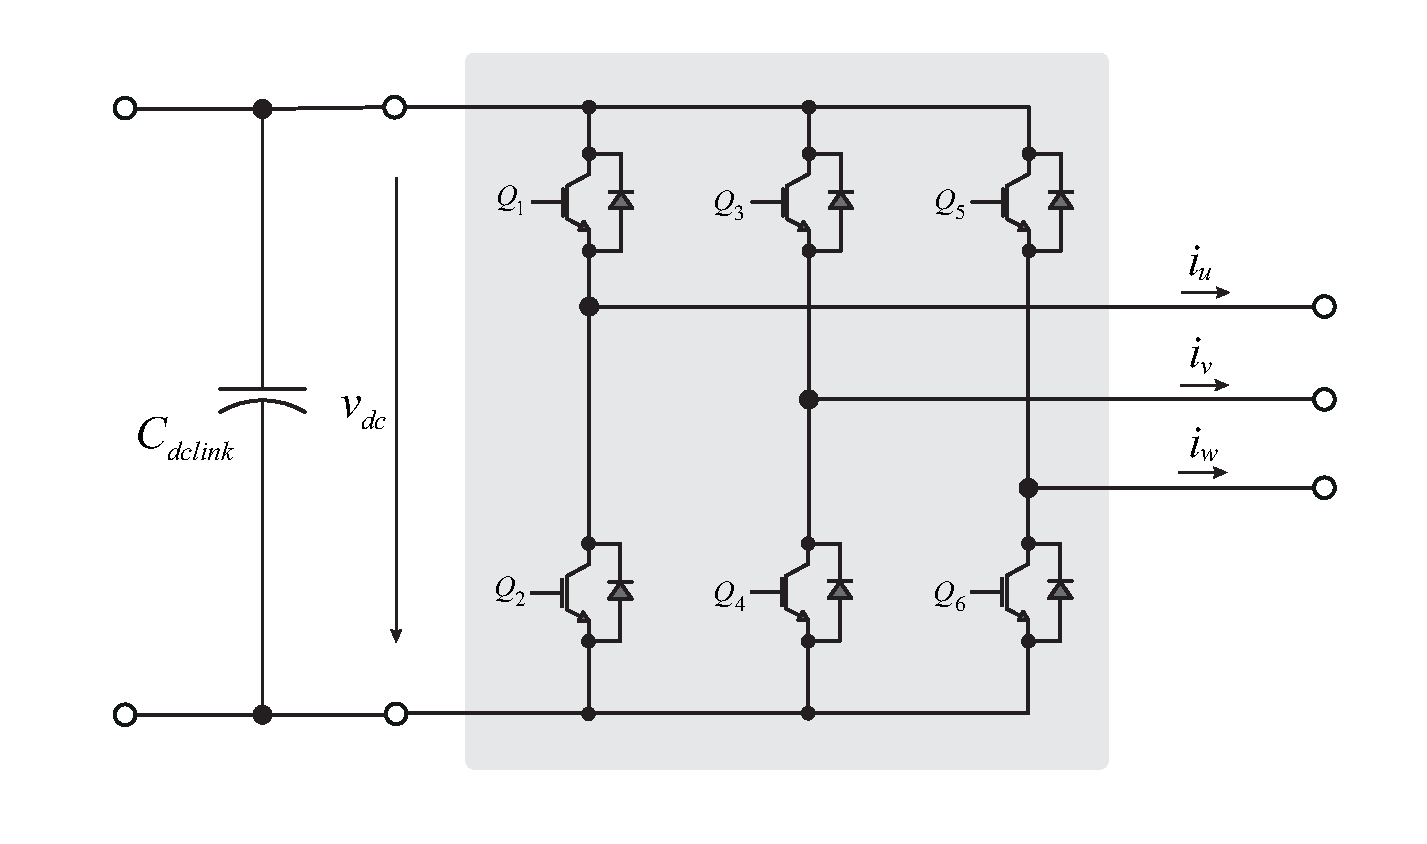
\includegraphics[width = 360pt, angle = 0, 
	keepaspectratio]{figures/electrical_layout/electrical_circuit_3.eps}
	\captionsetup{width=0.5\textwidth, font=small}	
	\caption{Inverter electrical layout principle.}
	\label{electrical_circuit_1}
\end{figure}

\section{Preliminary Simulation Results}
This section shows some preliminary simulation results which have been performed in order to determine the main physical quantities used to design and sizing the hardware components of the inverter and to proof the feasibility of the control system architecture in term of sampling time and switching frequency.

Simulations have been implemented using the following data:
\begin{itemize}
	\item[--] nominal speed : $n = \SI{2291}{\per\minute}$, which results in a fundamental frequency of $f_e = \SI{1184}{\hertz}$;
	\item[--] nominal load current : $i_{load}^{nom} = \SI{64}{\ampere}$;	
	\item[--] nominal load torque : $\tau_e = \SI{64}{\newton\meter}$;
	\item[--] rotor position observer based on Back-EMF if the PMSM;
	\item[--] modulation strategy based on space vector at fixed switching frequency of $f_{sw}=\SI{25}{\kilo\hertz}$;
	\item[--] DC-link capacitance of $C_{dclink}=\SI{90}{\micro\farad}$.
\end{itemize}
Figure~\ref{psim_results_fig_12} to Figure~\ref{psim_results_fig_56} show the main motor and inverter quantities involved into the preliminary design of the inverter hardware components.
\begin{figure}[H]
	\centering
	\begin{subfigure}{0.5\textwidth}
		\centering
		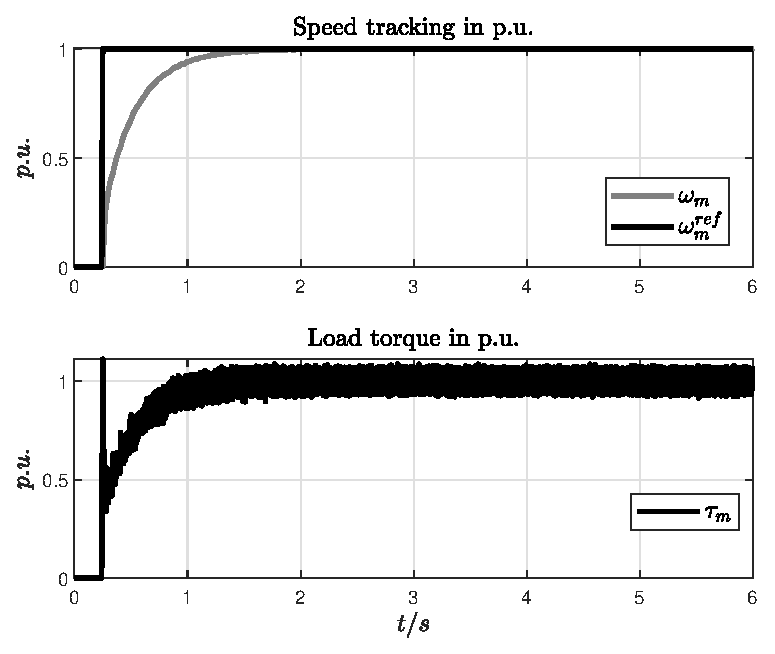
\includegraphics[width = 200pt, angle = 0, 
		keepaspectratio]{figures/preliminary_simulation_results/sim_results_preliminary_fig_1.eps}
		\captionsetup{width=0.65\textwidth, font=footnotesize}	
		\caption{Speed tracking performance in per unit.}
		\label{psim_results_fig_1}
	\end{subfigure}%
	\begin{subfigure}{.5\textwidth}
		\centering
		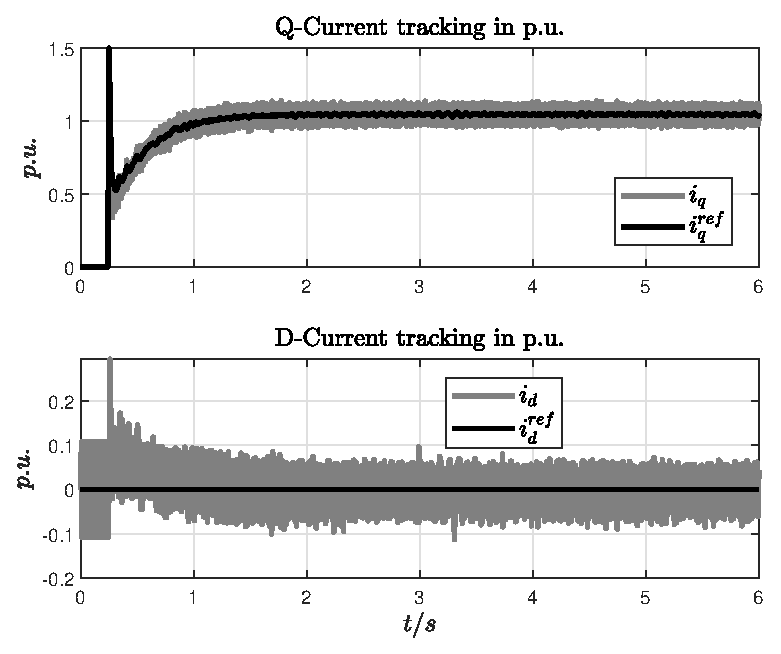
\includegraphics[width = 200pt, angle = 0, 
		keepaspectratio]{figures/preliminary_simulation_results/sim_results_preliminary_fig_2.eps}
		\captionsetup{width=0.65\textwidth, font=footnotesize}	
		\caption{Quadrature and direct currents tracking performance in per unit..}
		\label{psim_results_fig_2}
	\end{subfigure}
	\captionsetup{width=0.5\textwidth, font=small}	
	\caption{Tracking performance}
	\label{psim_results_fig_12}
\end{figure}
\begin{figure}[H]
	\centering
	\begin{subfigure}{0.5\textwidth}
		\centering
		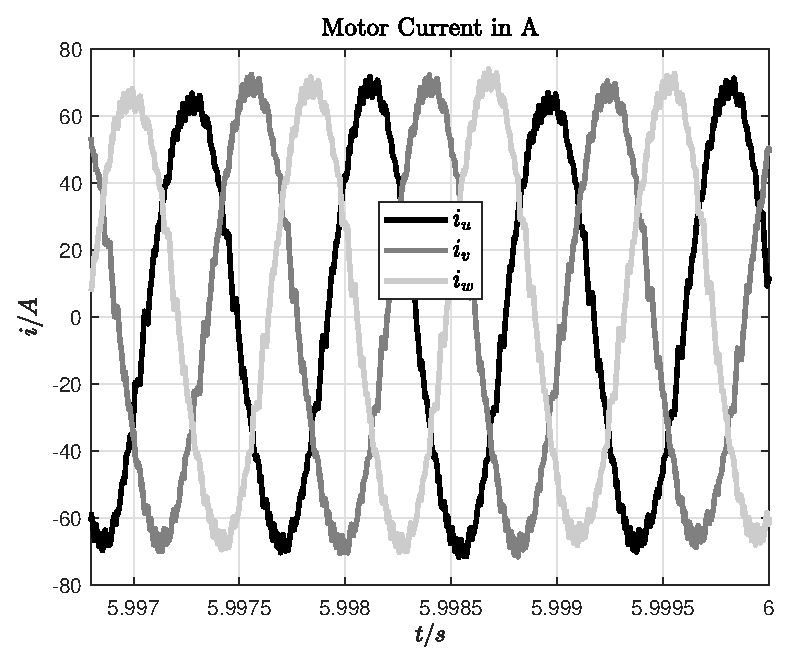
\includegraphics[width = 200pt, angle = 0, 
		keepaspectratio]{figures/preliminary_simulation_results/sim_results_preliminary_fig_3.eps}
		\captionsetup{width=0.65\textwidth, font=footnotesize}	
		\caption{Inverter three phase currents in SI.}
		\label{psim_results_fig_3}
	\end{subfigure}%
	\begin{subfigure}{.5\textwidth}
		\centering
		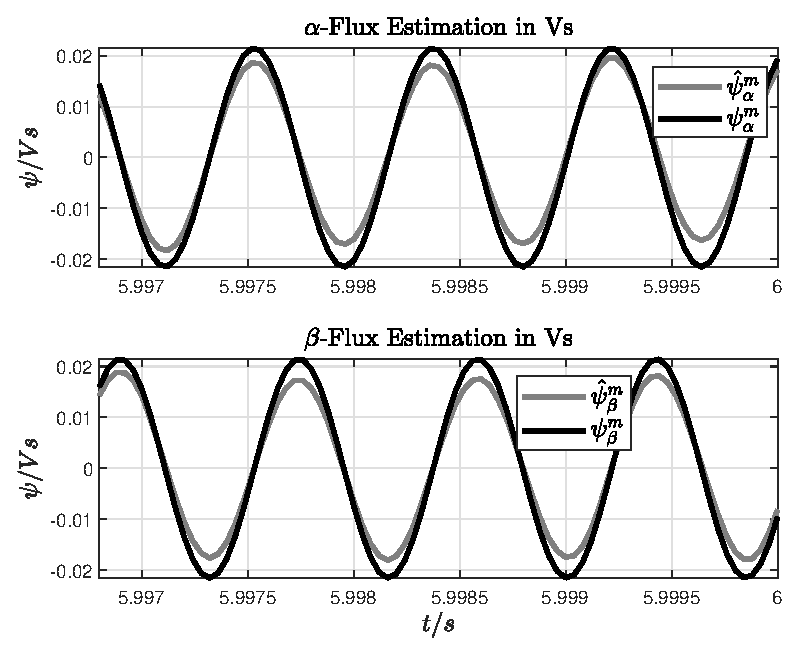
\includegraphics[width = 200pt, angle = 0, 
		keepaspectratio]{figures/preliminary_simulation_results/sim_results_preliminary_fig_4.eps}
		\captionsetup{width=0.65\textwidth, font=footnotesize}	
		\caption{$\alpha$ and $\beta$ fluxes from PMSM and from Back EMF observer in SI.}
		\label{psim_results_fig_4}
	\end{subfigure}
	\captionsetup{width=0.5\textwidth, font=small}	
	\caption{Inverter currents and fluxes observer performance}
	\label{psim_results_fig_34}
\end{figure}
\begin{figure}[H]
	\centering
	\begin{subfigure}{0.5\textwidth}
		\centering
		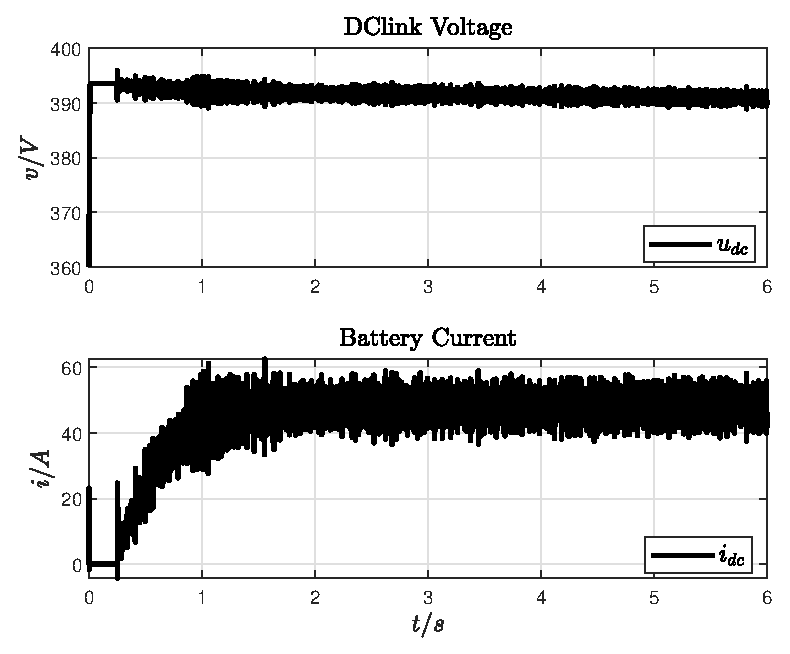
\includegraphics[width = 200pt, angle = 0, 
		keepaspectratio]{figures/preliminary_simulation_results/sim_results_preliminary_fig_5.eps}
		\captionsetup{width=0.65\textwidth, font=footnotesize}	
		\caption{DC-link voltage and battery current in SI.}
		\label{psim_results_fig_5}
	\end{subfigure}%
	\begin{subfigure}{.5\textwidth}
		\centering
		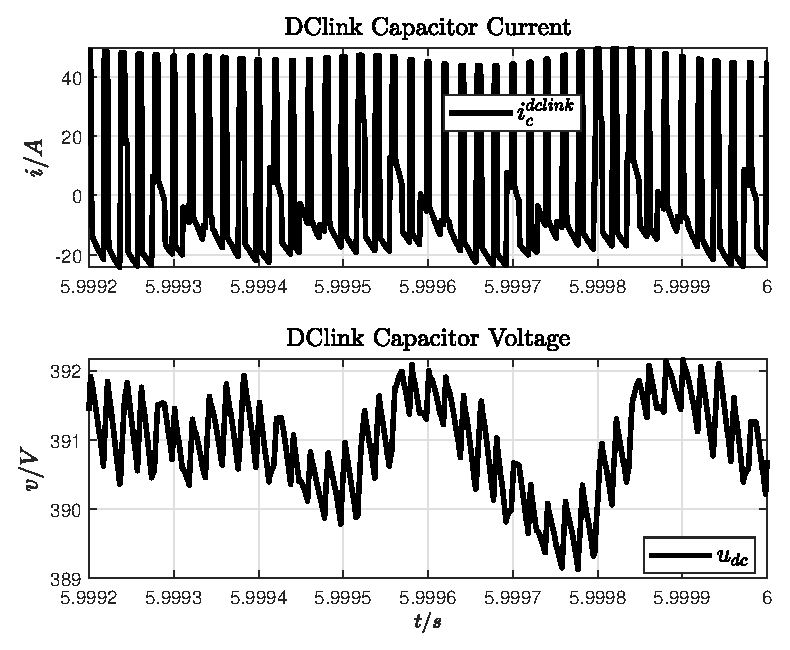
\includegraphics[width = 200pt, angle = 0, 
		keepaspectratio]{figures/preliminary_simulation_results/sim_results_preliminary_fig_6.eps}
		\captionsetup{width=0.65\textwidth, font=footnotesize}	
		\caption{DC-link capacitor voltage and current (\SI{24}{\ampere} RMS)in SI.}
		\label{psim_results_fig_6}
	\end{subfigure}
	\captionsetup{width=0.5\textwidth, font=small}	
	\caption{Battery voltage and current in SI. DC-link capacitor voltage and current in SI}
	\label{psim_results_fig_56}
\end{figure}

\section{Preliminary Components Selection}
As result of an extensive market search for product availability and thermal performance evaluation the selected  component is here illustrated. According to Table~\ref{M50C35EEE9KV_table_4} the component \textbf{CAB016M12FM3} has been selected, and thermal performance will be presented as well, see Table~\ref{inverter_sizing_1}.

\begin{figure}[H]
	\centering
	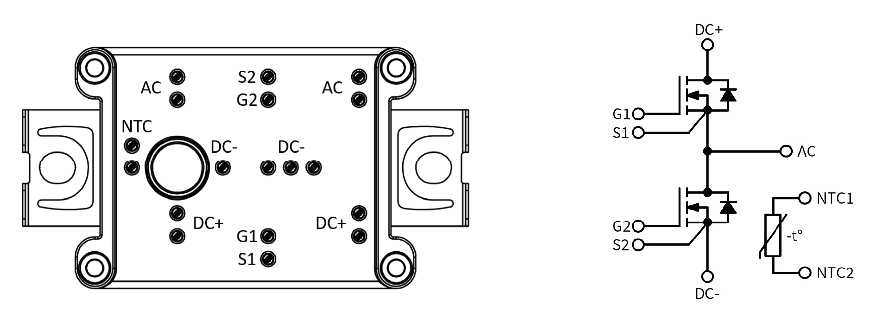
\includegraphics[width = 300pt, angle = 0, 
	keepaspectratio]{figures/CAB016_module/CAB016_module_package.eps}
	\captionsetup{width=0.5\textwidth, font=small}	
	\caption{CAB016 module description.}
\end{figure}
\begin{figure}[H]
	\centering
	\includegraphics[width = 450pt, angle = 0, 
	keepaspectratio]{figures/CAB016_module/CAB016_module_package_dimension_1.eps}
	\captionsetup{width=0.5\textwidth, font=small}	
	\caption{CAB016 module size description.}
\end{figure}

\begin{table}[H]
	%	\footnotesize
	\small
	\begin{center}	
		\begin{tblr}{p{0.75\linewidth}|p{0.25\linewidth}}
			\textbf{Quantity} & \textbf{Nominal value} \\
			\hline
			Drain-Source Voltage			& $V_{DSmax} = \SI{1200}{\volt}$ \\	
			Continuos DC (RMS) Drain Current	& $I_{D} = \SI{80}{\ampere}$ \\	
			Maximum Junction Temp. Switching Conditions	& $T_{jop} = \SI{150}{\celsius}$ \\	
			Drain-Source On-State Resistance ($T_j=\SI{125}{\celsius}$) & $R_{DSon} = \SI{21.6}{\milli\ohm}$ \\
			Terminal Resistance ($T_j=\SI{125}{\celsius}$) & $R_{term} = \SI{2.06}{\milli\ohm}$ \\
			Turn-On Switching Energy ($R_g^{on}=\SI{4}{\ohm}$, $T_j=\SI{125}{\celsius}$, $u_{dc}=\SI{600}{\volt}$, $i_{d}=\SI{80}{\ampere}$) & $E_{on}=\SI{1.16}{\milli\joule}$ \\
			Turn-Off Switching Energy ($R_g^{off}=\SI{4}{\ohm}$, $T_j=\SI{125}{\celsius}$, $u_{dc}=\SI{600}{\volt}$, $i_{d}=\SI{80}{\ampere}$) & $E_{off}=\SI{0.54}{\milli\joule}$ \\
			Reserve Recovery Energy ($T_j=\SI{125}{\celsius}$, $u_{dc}=\SI{600}{\volt}$, $i_{d}=\SI{80}{\ampere}$) & $E_{rr}=\SI{0.075}{\milli\joule}$ \\
			MOSFET Thermal Resistance, Junction to Heatsink & $R_{jh}=\SI{0.642}{\celsius\per\watt}$ \\
			\hline
		\end{tblr}
	\end{center}
	\captionsetup{width=.5\textwidth, font=small}
	\caption{CAB016M12FM3 Main Datasheet Parameters.}
	\label{}
\end{table}	

The estimated power losses, for the selected component, are reported in Tables~\ref{inverter_sizing_1} and they have been evaluated at the maximum operative working condition in order to extrapolate the maximum junction temperature.

\begin{table}[H]
	%	\footnotesize
	\small
	\begin{center}	
		\begin{tblr}{p{0.2\linewidth}|p{0.1\linewidth}|p{0.1\linewidth}|p{0.1\linewidth}|p{0.1\linewidth}|p{0.1\linewidth}}
			\textbf{Model} & $P_{sw}^{switch}$ & $P_{cond}^{switch}$ & $P_{loss}^{switch}$ & $P_{loss}^{tot}$ & $T_{J}^{max}$ \\
			\hline
			\textbf{CAB016M12FM3} & \SI{26.0}{\watt} & \SI{10}{\watt} & \SI{36.0}{\watt} & \SI{216}{\watt} & \SI{110}{\celsius} \\
			\hline
		\end{tblr}
	\end{center}
	\captionsetup{width=.5\textwidth, font=small}
	\caption{Preliminary power losses evaluation and maximum reached junction temperature.}
	\label{inverter_sizing_1}
\end{table}	

\subsection{DC-link Capacitor}
The initial selection of the DC-link capacitor value starts from the consideration to have a switching voltage ripple around $\Delta v_{dc} \approx \SI{1}{\volt}$ peak to peak. The preliminary capacitor is here selected using the component \textbf{C4AQLBU4560A1WK} from KEMET.

The component \textbf{C4AQLBU4560A1WK} has the following characteristics:
\begin{itemize}
	\item[--] Capacitance: $C=15 \times \SI{5.6}{\micro\farad}$;
	\item[--] Nominal current: $I_c^{nom}=15 \times \SI{6.8}{\ampere}$ (RMS) at \SI{75}{\celsius};
	\begin{itemize}
		\item[--] expected current: $i_c=\SI{24}{\ampere}$ (RMS)
	\end{itemize}
	\item[--] Nominal voltage: $V_C^{nom}=\SI{500}{\volt} - DC$;
	\item[--] Dimensions: $L=\SI{32}{\milli\meter}$, $T=\SI{11}{\milli\meter}$, $H=\SI{20}{\milli\meter}$;
	\item[--] Weight: $Wg=15 \times \SI{8}{\gram} = \SI{120}{\gram} $.
\end{itemize}

For preliminary design, it is assumed that the maximum junction temperature at nominal condition should not exceed the value of $T_J=\SI{125}{\celsius}$ supposing a constant heat sink temperature of $T_H=\SI{84}{\celsius}$.


\subsection{Electro-thermal Simulation Results}
\noindent  The power losses will be evaluated with the following rating condition:

\begin{table}[H]
	%	\footnotesize
	\small
	\begin{center}	
		\begin{tblr}{p{0.75\linewidth}|p{0.25\linewidth}}
			\textbf{Quantity} & \textbf{value} \\
			\hline
			Load current			& $I_m = \SI{45}{\ampere}$ (RMS) \\	
			Load voltage	& $U_{m} = \SI{262}{\ampere}$ (ph-ph RMS) \\	
			Load power factor	& $\cos(\phi) = \SI{0.9}{}$ \\	
			Load fundamental frequency & $f_{load} = \SI{1250}{\hertz}$ \\
			Inverter switching frequency & $f_{sw} = \SI{25}{\kilo\hertz}$ \\
			DC-link voltage & $v_{dc}=\SI{400}{\volt}$ \\
			External gate ON resistance & $R_g^{on}=\SI{6}{\ohm}$ \\			
			External gate OFF resistance & $R_g^{off}=\SI{6}{\ohm}$ \\
			Turn-On Switching Energy ($R_g^{on}=\SI{6}{\ohm}$, $T_j=\SI{125}{\celsius}$, $u_{dc}=\SI{600}{\volt}$, $i_{d}=\SI{80}{\ampere}$) & $E_{on}=\SI{1.56}{\milli\joule}$ \\
			Turn-Off Switching Energy ($R_g^{off}=\SI{6}{\ohm}$, $T_j=\SI{125}{\celsius}$, $u_{dc}=\SI{600}{\volt}$, $i_{d}=\SI{80}{\ampere}$) & $E_{off}=\SI{0.84}{\milli\joule}$ \\
			Reserve Recovery Energy ($T_j=\SI{125}{\celsius}$, $u_{dc}=\SI{600}{\volt}$, $i_{d}=\SI{80}{\ampere}$) & $E_{rr}=\SI{0.075}{\milli\joule}$ \\
			MOSFET Thermal Resistance, Junction to Heatsink (per MOSFET) & $R_{jh}=\SI{0.642}{\celsius\per\watt}$ \\
			Thermal Interface Material (per MOSFET) & $R_{TIM}=\SI{0.5}{\celsius\per\watt}$ \\
			MOSFET Thermal Resistance, Heatsink to Ambient (per MOSFET) & $R_{ha}=\SI{1.88}{\celsius\per\watt}$ \\
			\hline
		\end{tblr}
	\end{center}
	\captionsetup{width=.5\textwidth, font=small}
	\caption{List of condition for the electro-thermal simulation.}
	\label{}
\end{table}	

Simulations have been carried out neglecting the thermal capacity of the heat-sink in order to evaluate the steady state temperature for different load conditions.
 \begin{figure}[H]
 	\centering
 	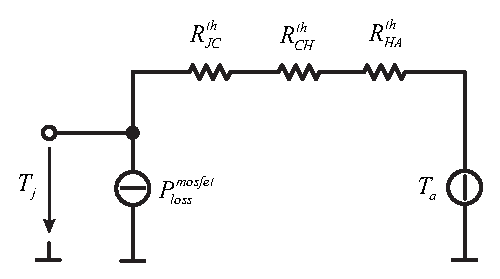
\includegraphics[width = 250pt, angle = 0, 
 	keepaspectratio]{figures/thermal_model/thermal_model_fig_1.eps}
 	\captionsetup{width=0.5\textwidth, font=small}	
 	\caption{Steady state thermal model of the single MOSFET component.}
 	\label{}
 \end{figure}

\begin{figure}[H]
	\centering
	\includegraphics[width = 450pt, angle = 0, 
	keepaspectratio]{figures/layout/layout_4.eps}
	\captionsetup{width=0.5\textwidth, font=small}	
	\caption{Preliminary design for electro/thermal simulation. In scale assembling layout: module+heatsink+dclink with weights.}
	\label{}
\end{figure}

\begin{figure}[H]
	\centering
	\begin{subfigure}{0.5\textwidth}
		\centering
		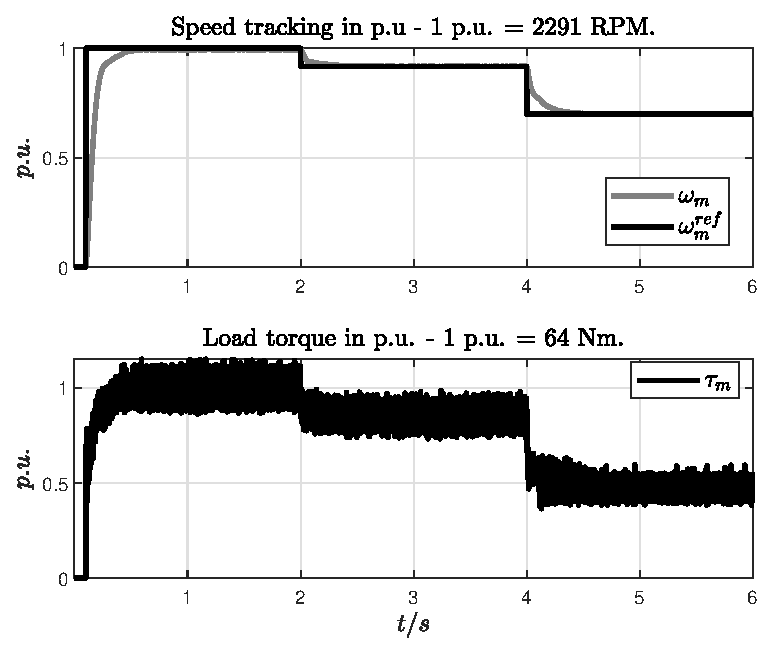
\includegraphics[width = 200pt, angle = 0, 
		keepaspectratio]{figures/thermal_analysis/case_1/sim_results_fig_1.eps}
		\captionsetup{width=0.85\textwidth, font=footnotesize}	
		\caption{Speed tracking performance in per unit (top) - Electromagnetic torque in per unit (bottom). At time $t=\SI{2}{\second}$ the speed reference change from \SI{2291}{\per\minute} to \SI{2102}{\per\minute} and at time $t=\SI{4}{\second}$ the speed reference change from \SI{2102}{\per\minute} to \SI{1600}{\per\minute}.}
		\label{}
	\end{subfigure}%
	\begin{subfigure}{.5\textwidth}
		\centering
		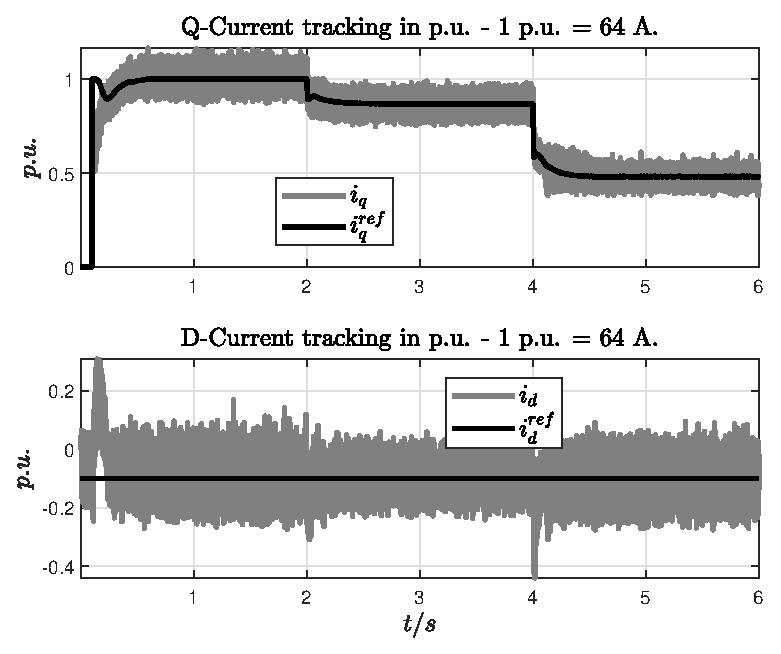
\includegraphics[width = 200pt, angle = 0, 
		keepaspectratio]{figures/thermal_analysis/case_1/sim_results_fig_2.eps}
		\captionsetup{width=0.85\textwidth, font=footnotesize}	
		\caption{Quadrature (top) and direct (bottom) currents tracking performance in per unit.\vspace{11mm}}
		\label{}
	\end{subfigure}
	\captionsetup{width=0.5\textwidth, font=small}	
	\caption{Electro-thermal simulation results at different loads.}
	\label{}
\end{figure}
\begin{figure}[H]
	\centering
	\begin{subfigure}{0.5\textwidth}
		\centering
		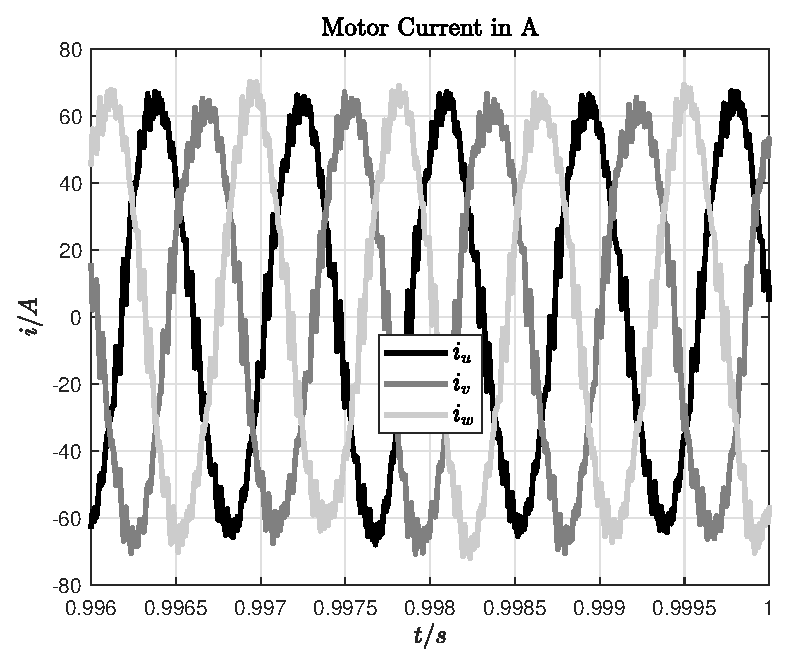
\includegraphics[width = 200pt, angle = 0, 
		keepaspectratio]{figures/thermal_analysis/case_1/sim_results_fig_3.eps}
		\captionsetup{width=0.5\textwidth, font=footnotesize}	
		\caption{Inverter three phase currents in SI, at nominal torque. \vspace{2mm}}
		\label{}
	\end{subfigure}%
	\begin{subfigure}{.5\textwidth}
		\centering
		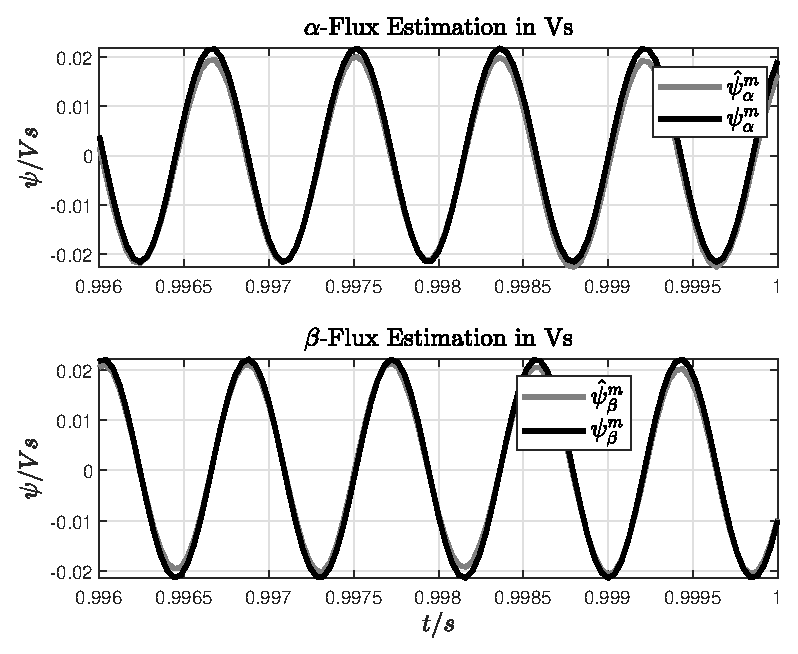
\includegraphics[width = 200pt, angle = 0, 
		keepaspectratio]{figures/thermal_analysis/case_1/sim_results_fig_4.eps}
		\captionsetup{width=0.5\textwidth, font=footnotesize}	
		\caption{$\alpha$ and $\beta$ fluxes from PMSM and from Back EMF observer in SI, at nominal torque.}
		\label{}
	\end{subfigure}
	\captionsetup{width=0.5\textwidth, font=small}	
	\caption{Electro-thermal simulation results at different loads.}
	\label{}
\end{figure}


\begin{figure}[H]
	\centering
	\begin{subfigure}{0.5\textwidth}
		\centering
		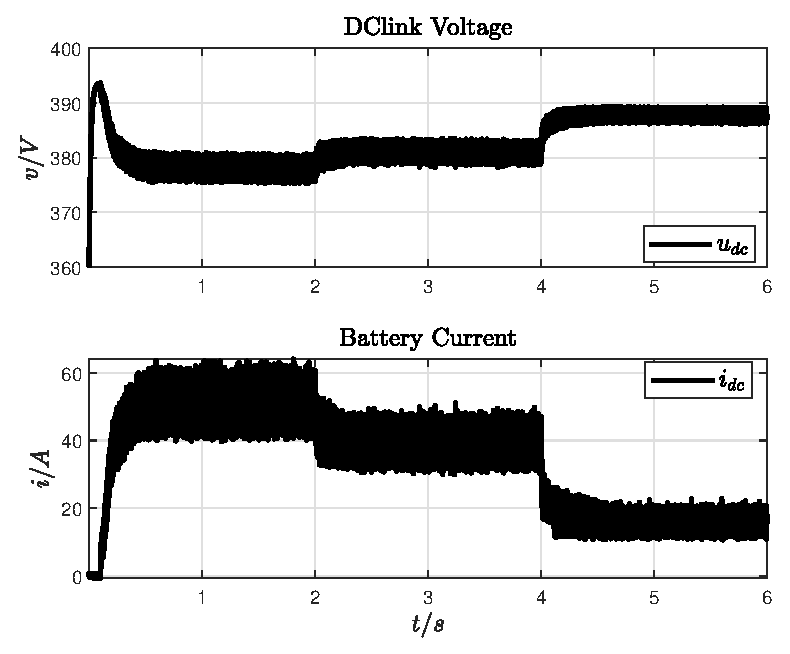
\includegraphics[width = 200pt, angle = 0, 
		keepaspectratio]{figures/thermal_analysis/case_1/sim_results_fig_5.eps}
		\captionsetup{width=0.85\textwidth, font=footnotesize}	
		\caption{DC-link voltage (top) and battery current in SI (bottom).\vspace{5mm}}
		\label{}
	\end{subfigure}%
	\begin{subfigure}{.5\textwidth}
		\centering
		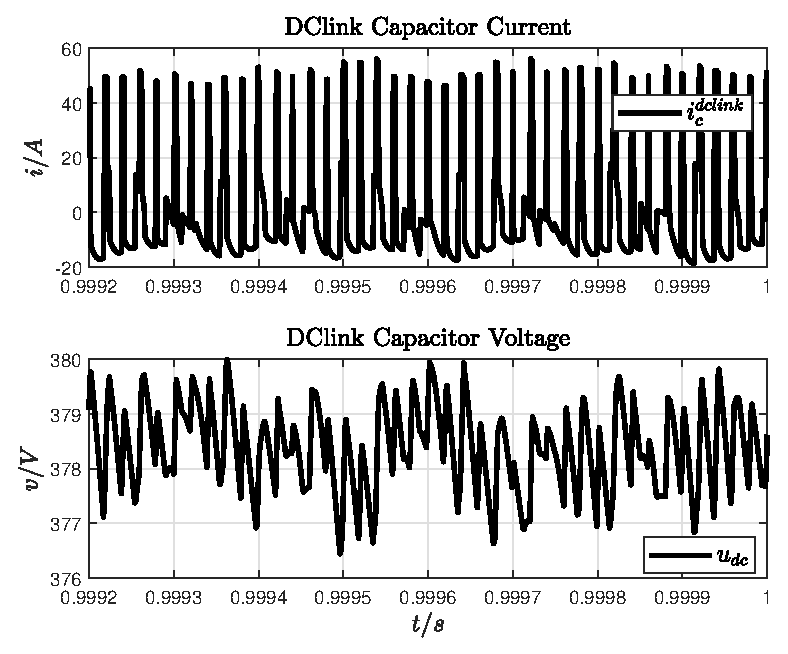
\includegraphics[width = 200pt, angle = 0, 
		keepaspectratio]{figures/thermal_analysis/case_1/sim_results_fig_6.eps}
		\captionsetup{width=0.85\textwidth, font=footnotesize}	
		\caption{DC-link capacitor voltage (bottom) and DC-link capacitor current (top) - internal capacitor current is $I_c=\SI{22.0}{\ampere}$ RMS in SI, at nominal torque.}
		\label{}
	\end{subfigure}
	\captionsetup{width=0.5\textwidth, font=small}	
	\caption{Electro-thermal simulation results at different loads.}
	\label{}
\end{figure}

\begin{figure}[H]
	\centering
	\begin{subfigure}{0.5\textwidth}
		\centering
		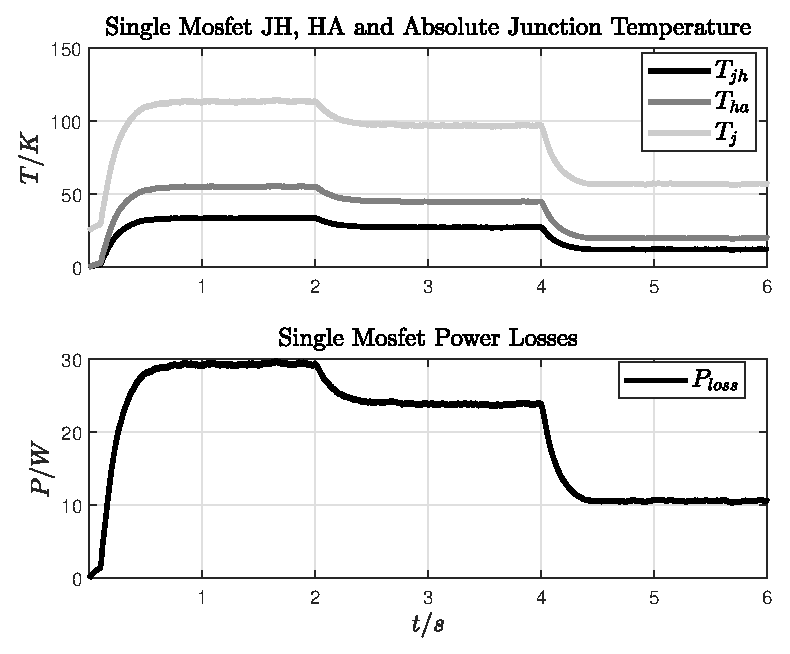
\includegraphics[width = 200pt, angle = 0, 
		keepaspectratio]{figures/thermal_analysis/case_1/sim_results_fig_7.eps}
		\captionsetup{width=0.85\textwidth, font=footnotesize}	
		\caption{MOSFET power losses (bottom), MOSFET junction temperature (top-light grey).}
		\label{}
	\end{subfigure}%
	\begin{subfigure}{.5\textwidth}
		\centering
		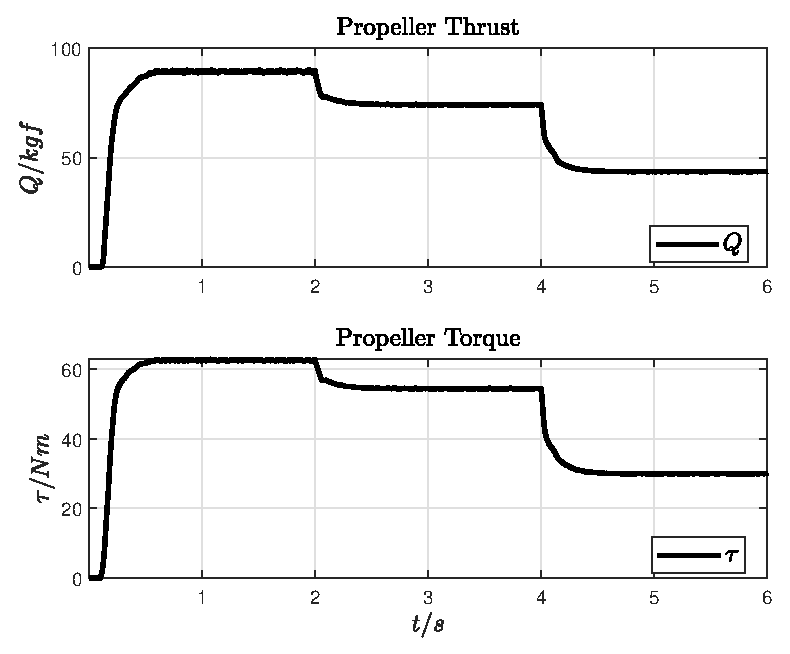
\includegraphics[width = 200pt, angle = 0, 
		keepaspectratio]{figures/thermal_analysis/case_1/sim_results_fig_8.eps}
		\captionsetup{width=0.85\textwidth, font=footnotesize}	
		\caption{Propeller thrust (top) and torque (bottom) with FLUXER PRO 63x22.}
		\label{}
	\end{subfigure}
	\captionsetup{width=0.5\textwidth, font=small}	
	\caption{Electro-thermal simulation results at different loads.}
	\label{}
\end{figure}
The CAB016 Module coupled with the Heatsink ALPHA-LT13070-35W can drive full load torque in continuos mode, as shown in the following thermal simulation (no thermal capacities are taken into account). The maximum MOSFET Junction temperature is always below than \SI{125}{\celsius} under an ambient temperature of \SI{25}{\celsius}: 
\begin{figure}[H]
	\centering
	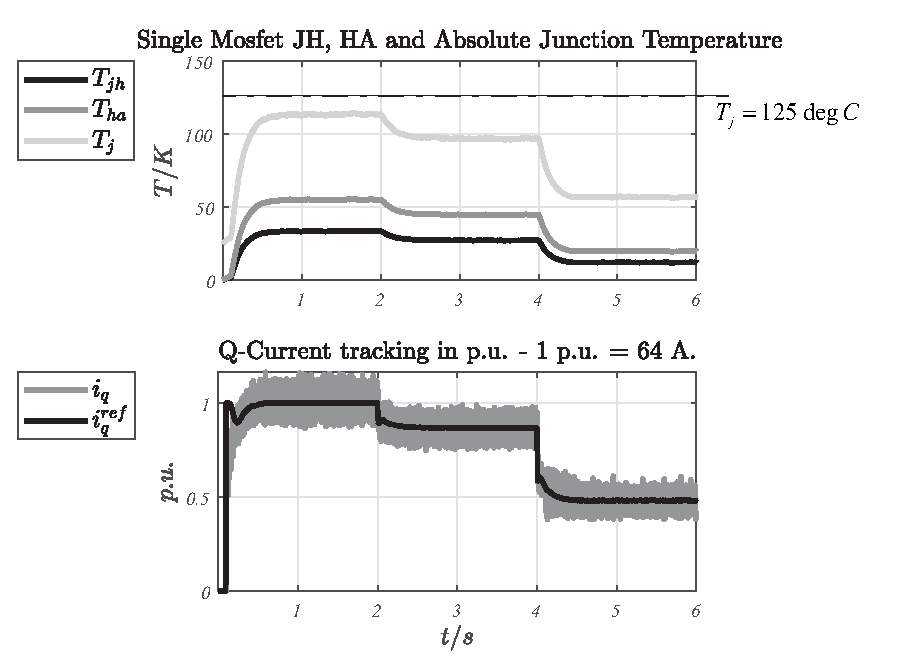
\includegraphics[width = 400pt, angle = 0, 
	keepaspectratio]{figures/thermal_analysis/case_1/sim_results_fig_9b.eps}
	\captionsetup{width=0.5\textwidth, font=small}	
	\caption{Simulation results: Motor current in per unit (bottom), MOSFET junction temperature (top-light grey).\vspace{3.5mm}}
\end{figure} 

The maximum continuative motor current which the CAB016 module is able to supply will be defined as the maximum motor current in which the Junction temperature of CAB016 module will rise up to $T_j^{max}=\SI{125}{\celsius}$ when $T_{ambient}=\SI{25}{\celsius}$. 
The evaluation will be done exploring by simulation three propeller working points as shown in the following table.

\begin{table}[H]
	%	\footnotesize
	\small
	\begin{center}	
		\begin{tblr}{p{0.3\linewidth}|p{0.3\linewidth}|p{0.3\linewidth}}
			\textbf{Rotor Speed}  & \textbf{Torque} & \textbf{Thrust} \\
			\hline
			\SI{2291}{\per\minute}	& \SI{64}{\newton\meter}	&	\SI{93}{\kilogram} \\		\SI{2102}{\per\minute}	& \SI{54.5}{\newton\meter}	&	\SI{75}{\kilogram} \\
			\SI{1600}{\per\minute}	& \SI{29.8}{\newton\meter}	&	\SI{43}{\kilogram} \\
			\hline
		\end{tblr}
	\end{center}
	\captionsetup{width=.5\textwidth, font=small}
	\caption{Performance evaluation of the with CAB016 Module with M50C35-EEE-9KV Motor, and FLUXER-PRO-63x22 Propeller.}
	\label{}
\end{table}	

\section{Dynamic thermal analysis}
In the following the thermal capacity of the ALPHA-LT13070-35W heatsink will be taken into account. The following figure shows the equivalent model of the “sandwich” CAB016M12FM3 module and ALPHA-LT13070-35W heatsink. The equivalent MOSFET surface where power is generated is in some around half of the heatsink surface. This effect is modelized splitting in two identical parts the \textbf{equivalent} thermal capacity and thermal resistance. 

Figure~\ref{thermal_model_fig_2} shows the equivalent thermal circuit seen by every single MOSFET is analysed,
\begin{figure}[H]
	\centering
	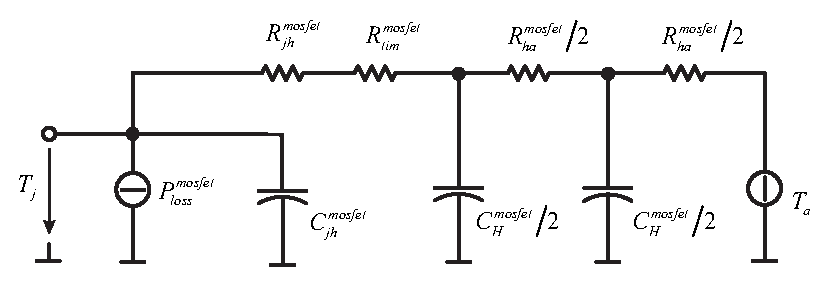
\includegraphics[width = 345pt, angle = 0, 
	keepaspectratio]{figures/thermal_analysis/thermal_model_fig_2.eps}
	\captionsetup{width=0.5\textwidth, font=small}	
	\caption{Equivalent thermal circuit (seen by a single MOSFET) where the thermal capacity of the heatsink has been included.}
	\label{thermal_model_fig_2}
\end{figure}
Considering Figure~\ref{thermal_analysis_1_V} as reference, the thermal impedances of the equivalent thermal network reported in Figure~\ref{thermal_model_fig_2} can be derived.
\begin{figure}[H]
	\centering
	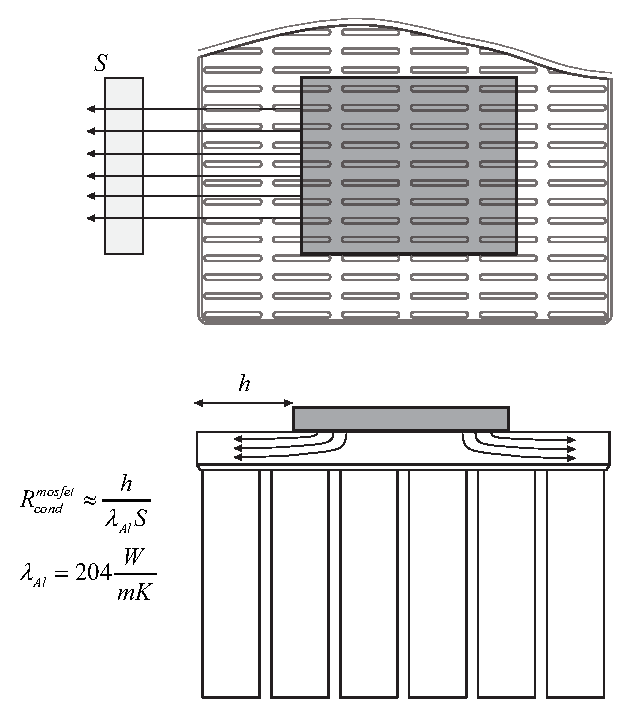
\includegraphics[width = 225pt, angle = 0, 
	keepaspectratio]{figures/thermal_analysis/thermal_analysis_1_V.eps}
	\captionsetup{width=0.5\textwidth, font=small}	
	\caption{CAB016M12FM3 case and ALPHA-LT13070-35W heatsink thermal exchange analysis.}
	\label{thermal_analysis_1_V}
\end{figure}
Let 
\begin{equation}
	R_{ha}\approx\SI{0.25}{\celsius\per\watt}
\end{equation}
be the whole nominal (from data-sheet) thermal impedance of the heat-sink. The equivalent thermal impedance seen by one MOSFET can be derived assuming a reduced  equivalent surface, seen by the MOSFET, as follows
\begin{equation}
	\begin{aligned}
		R_{cond}^{mosfet} &\approx\SI{0.35}{\celsius\per\watt} \\[6pt]
		R_{ha}^{mosfet} &\approx 6\cdot R_{ha} + R_{cond}^{mosfet} \approx \SI{2}{\celsius\per\watt}
	\end{aligned}
\end{equation}
The total equivalent thermal impedance seen by an MOSFET from junction to ambient can be represented as follows
\begin{equation}
	\begin{aligned}
	R_{ja}^{mosfet} &\approx R_{jh}^{mosfet} + R_{tim}^{mosfet}+R_{ha}^{mosfet} \approx\SI{3.3}{\celsius\per\watt}
	\end{aligned}
\end{equation}
The equivalent heat capacities of the mosfet and of the heat-sink are as follows
\begin{equation}
	\begin{aligned}
		C_H^{mosfet} &=\SI{47.8}{\joule\per\kelvin} \\[6pt]
		C_{jh}^{mosfet} &=\SI{0.025}{\joule\per\kelvin}
	\end{aligned}
\end{equation}

Dynamic thermal simulation of the CAB016M12FM3 module assuming $R_{JA}^{th}=\SI{3.3}{\kelvin\per\watt}$ (thermal resistance seen by the single individual MOSFET) and $T_a=\SI{30}{\celsius}$.
\begin{figure}[H]
	\centering
	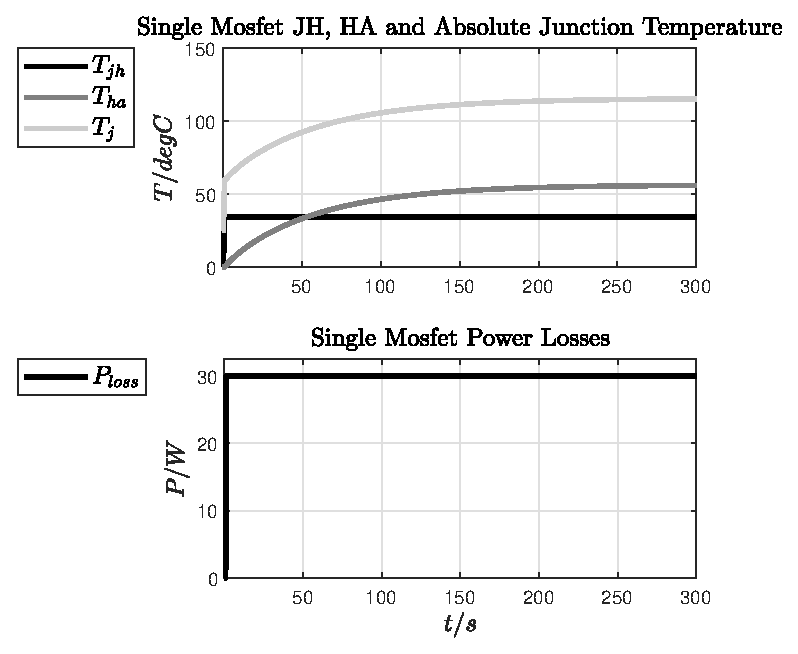
\includegraphics[width = 265pt, angle = 0, 
	keepaspectratio]{figures/thermal_analysis/sim_results_thermal_fig_1.eps}
	\captionsetup{width=0.75\textwidth, font=small}	
	\caption{Thermal response of the ALPHA-LT13070-35W heatsink seen by a single MOSFET for the case of $P_{loss}^{mosfet}=\SI{30}{\watt}$ - case for maximum continuative current of \SI{45}{\ampere} (RMS). Top Figures shows the Junction temperature (light grey) of a single MOSFET during time response.}
\end{figure}



\chapter{PMSM Control Architectures}
\section{Introduction}
In the following sections different control approaches will be investigated. The traditional vector control based on rotor flux estimation is used as first approach in order to obtain a design layout for components selection and minimum required microcontroller performance. Additional control strategies like model predictive control will be investigated.

For the purpose of modelization of the \textit{plant} as well as of the \textit{control system} in \textit{Simulink/Simscape} ambient, two different representations are adopted:
\begin{itemize}
	\item[--] system representation in continuous time domain with parameters in SI unit for plant models implementation;
	\item[--] system representation in discrete time domain with parameters in per unit for control systems (controllers, state observers, model based controllers, etc.) implementation.	
\end{itemize}

\subsection{Nomenclature}	
Here, a list of used symbols:
\begin{itemize}
	\item[--] $s.r.f.$: stationary reference frame;
	\item[--] $r.r.f.$: rotor reference frame;
	\item[--] $r.r.f.-\omega_0$: rotating reference frame at $\omega_0$;	
	\item[--] $p$: number of pole pairs;
	\item[--] $\omega_m$: mechanical rotor speed $\Big[\SI{}{\radian\per\second}\Big]$;
	\item[--] $\omega$ : electrical rotor speed $\Big[\SI{}{\radian\per\second}\Big]$;
	\item[--] $\vartheta$ : electrical rotor position $\Big[\SI{}{\radian}\Big]$;
	\item[--] $\vartheta_{emf}$ : electrical rotor position derived from rotor fluxes $\Big[\SI{}{\radian}\Big]$;
	\item[--] $\tau_m$ : electromagnetic torque $\Big[\SI{}{\newton\meter}\Big]$;
	\item[--] $i_\alpha$ : direct current in $s.r.f.$ $\Big[\SI{}{\ampere}\Big]$;
	\item[--] $i_\beta$ : quadrature current in $s.r.f.$ $\Big[\SI{}{\ampere}\Big]$;
	\item[--] $i_d$ : direct current in $r.r.f.$ $\Big[\SI{}{\ampere}\Big]$;
	\item[--] $i_q$ : quadrature current in $r.r.f.$ $\Big[\SI{}{\ampere}\Big]$;
	\item[--] $\psi_d^s=\psi_d^r+i_dL_d$ : direct flux $\Big[\SI{}{\weber}\Big]$;	
	\item[--] $\psi_q^s=\psi_q^r+i_qL_q$ : quadrature flux $\Big[\SI{}{\weber}\Big]$;	
	\item[--] $\psi_{\alpha}^s=\psi_{\alpha}^r+i_{\alpha}L_{s}$ : $\Big[\SI{}{\weber}\Big]$;	
	\item[--] $\psi_{\beta}^s=\psi_{\beta}^r+i_{\beta}L_{s}$ : $\Big[\SI{}{\weber}\Big]$;		
	\item[--] $\psi^m$ : permanent magnet linkage flux $\Big[\SI{}{\weber}\Big]$;		
	\item[--] $u_d$ : direct motor terminal voltage in $r.r.f.$ $\Big[\SI{}{\volt}\Big]$;
	\item[--] $u_q$ : quadrature motor terminal voltage in $r.r.f.$ $\Big[\SI{}{\volt}\Big]$;
	\item[--] $u_\alpha$ : direct motor terminal voltage in $s.r.f.$ $\Big[\SI{}{\volt}\Big]$;
	\item[--] $u_\beta$ : quadrature motor terminal voltage in $s.r.f.$ $\Big[\SI{}{\volt}\Big]$;
\end{itemize}

\subsection{Normalization and vector current control implementation.}
The per unit representation of a dynamic system passes through the \textit{normalization} process, which can be described as follows
\begin{itemize}
	\item[--] Reference quantities
	\begin{itemize}
		\item[--] $u_{bez}$ : peak phase voltage (at no-load, at nominal rotor speed $\omega_m^{nom}$) of the motor in $\SI{}{\volt}$;
		\item[--] $i_{bez}$ : peak phase nominal current of the motor in $\SI{}{\ampere}$ and can be derived from parameter $\tau_m^{nom}$ (Nominal Torque) as follows
		\begin{equation}
			i_{bez} = \frac{2}{3}\frac{\tau_m^{nom}}{p\,\psi_{bez}} \qquad\text{we consider $i_d=0$ control};
		\end{equation}
		\item[--] $\omega_m^{nom}$ : nominal mechanical rotor speed of the motor in $\SI{}{\radian\per\second}$;
		\item[--] $\omega_{bez} = p\,\omega_m^{nom}$ : nominal electrical speed of the motor in $\SI{}{\radian\per\second}$;
		\item[--] $X_{bez} = u_{bez}/i_{bez}$ : reference electrical impedance of the motor in $\SI{}{\ohm}$;
		\item[--] $L_{bez} = X_{bez}/\omega_{bez}$ : reference inductance of the motor in $\SI{}{\henry}$;
		\item[--] $\psi_{bez} = u_{bez}/\omega_{bez}$ : reference flux of the motor in $\SI{}{\weber}$.
	\end{itemize}
	\item[--] Per unit quantities
	\begin{itemize}
		\item[--] $R_s^{norm} = R_s/X_{bez}$ : per unit of the phase resistance;
		\item[--] $L_s^{norm} = L_s/L_{bez}$ : per unit of $L_s$ inductance;
		\item[--] $\omega^{norm} = p\omega_m/\omega_{bez}$ : per unit of the electrical speed;		
		\item[--] $i^{norm} = i/i_{bez}$ : per unit of $i$ current;
		\item[--] $u^{norm} = u/u_{bez}$ : per unit of $u$ voltage;
		\item[--] $\psi_m^{norm} = \psi^m/\psi_{bez} = 1$ : per unit of the linkage permanent magnet flux.
	\end{itemize}	 
\end{itemize}

\section{Vector Control based on Flux Observers}
A preliminary control architecture, based on direct and quadrature current control obtained via Clarke and Park transformation is assumed. The rotor position, needed for Park transformation is estimated by Luenberger observer. The equations of the back EMF model are used to estimated the stator linkage fluxes respect to the stationary reference frame (obtaining the components $\hat{\psi}_{\alpha}(t)$ and $\hat{\psi}_{\beta}(t)$). From the flux components $\hat{\psi}_{\alpha}(t)$ and $\hat{\psi}_{\beta}(t)$ the rotor position is calculated via $\atantwo()$ function, obtaining the estimated rotor phase $\hat{\vartheta}_{bemf}(t)$. The rotor phase $\hat{\vartheta}_{bemf}(t)$ is additionally filtered and time derivate using the double integrator observer. In the following control schematic layouts will be presented.

The current vector control can be written as follows:
\begin{mybox}
	\begin{equation}
		\left\lbrace \begin{aligned}
			&i_q^{ref} = k_p^w\Big(\omega^{ref} - \omega\Big) + i_{q}^{i} \\[6pt]
			&\frac{d}{dt} i_{q}^{i}= k_i^w\Big(\omega^{ref} - \omega\Big) \\[6pt]
			&u_d^{ctrl} =  k_p^i\Big(i_d^{ref} - i_d\Big) + u_d^i - \omega\hat{\psi}_q - \omega L_q i_q \\[6pt]
			&\frac{d}{dt} u_d^i= k_i^i\Big(i_d^{ref} - i_d\Big)\\[6pt]
			&u_q^{ctrl} =  k_p^i\Big(i_q^{ref} - i_q\Big) + u_d^i + \omega\hat{\psi}_d - \omega L_d i_d \\[6pt]
			&\frac{d}{dt} u_q^i= k_i^i\Big(i_q^{ref} - i_q\Big)
		\end{aligned}\right. 
	\end{equation}
\end{mybox}
where for the sake of clarity equations are kept in continuous time domain and the superscript $\Big(\Big)^{norm}$ is omitted. Figure~\ref{vector_pi_1} shows the equivalent diagram representation comprehensive of the vector saturation and corresponding integrals anti-windup. 
\begin{figure}[H]
	\centering
	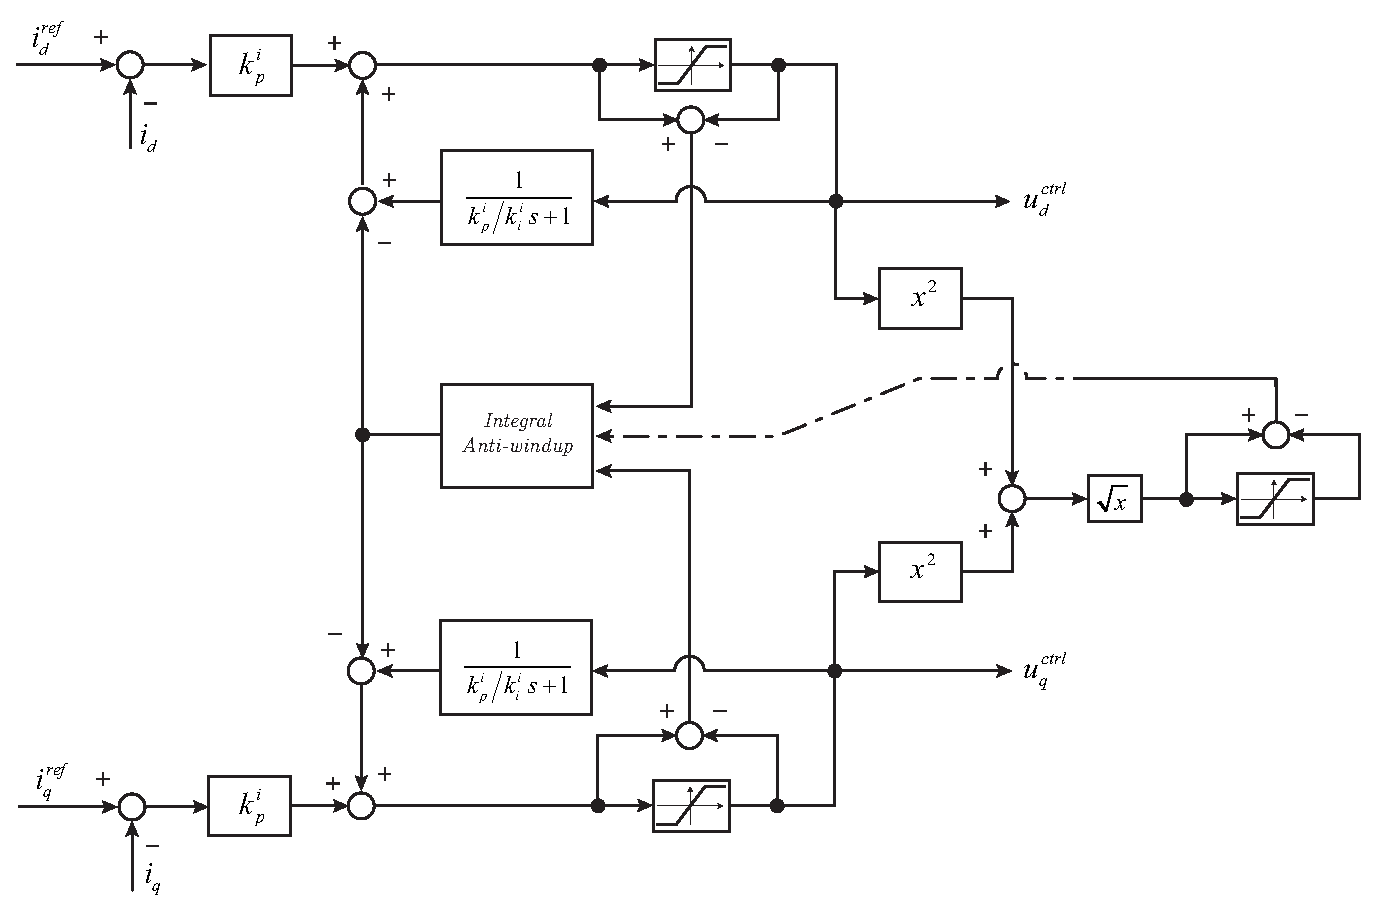
\includegraphics[height= 300pt, angle = 0, 
	keepaspectratio]{figures/control_layout/vector_pi_2.eps}
	\captionsetup{width=0.5\textwidth, font=small}	
	\caption{Vector PI with components and magnitude saturation with anti-windup diagram.}
	\label{vector_pi_1}
\end{figure}


\subsection{Back EMF based Observer}
Define
\begin{align}
	&\abs{\psi^m} = 1\qquad\text{(in per unit parameter)} \label{emf_state_obse_eq1} \\[6pt]
	&\Big(\psi_{\alpha}^r\Big)^* = \abs{\psi^m}\cos\vartheta = \psi^m\cos\vartheta \label{emf_state_obse_eq2} \\[6pt]
	&\Big(\psi_{\beta}^r\Big)^* = \abs{\psi^m}\sin\vartheta = \psi^m\sin\vartheta \label{emf_state_obse_eq3}
\end{align}
The flux state observer can be written as follows
\begin{align}
	\frac{d\hat{\psi}_{\alpha}^s}{dt} &= -R_s i_{\alpha} + u_{\alpha} + k_\psi \Big(\psi^m\cos\hat{\vartheta}-\hat{\psi}_{\alpha}^r\Big) \label{emf_state_obse_eq4} \\[6pt]
	\frac{d\hat{\psi}_{\beta}^s}{dt} &= -R_s i_{\beta} + u_{\beta} + k_\psi \Big(\psi^m\sin\hat{\vartheta}-\hat{\psi}_{\beta}^r\Big) \label{emf_state_obse_eq5}
\end{align}
where
\begin{align}
	\hat{\psi}_{\alpha}^r = \hat{\psi}_{\alpha}^s -L_s i_{\alpha} \label{emf_state_obse_eq6} \\[6pt]
	\hat{\psi}_{\beta}^r = \hat{\psi}_{\beta}^s -L_s i_{\beta} \label{emf_state_obse_eq7}
\end{align}
The mechanical state observer\footnote{see \S~\ref{state_observer_theory}} can be written as follows
\begin{align}
	\frac{d\hat{\vartheta}}{dt} &= \hat{\omega} + k_{\vartheta}\Big(\hat{\vartheta}_{emf} - \hat{\vartheta}\Big) \label{emf_state_obse_eq8} \\[6pt]
	\frac{d\hat{\omega}}{dt} &= k_{\omega}\Big(\hat{\vartheta}_{emf} - \hat{\vartheta}\Big) \label{emf_state_obse_eq9}
\end{align}
where 
\begin{align}
	\hat{\vartheta}_{emf} = \atantwo\big(\hat{\psi}_{\beta}^r,\,\hat{\psi}_{\alpha}^r\big) \label{emf_state_obse_eq10}
\end{align}
See also the control layout diagram depicted in Figure~\ref{pmsm_sv_ctrl_scheme_1}.

For practical implementation the equations
\begin{align}
	\frac{d\hat{\psi}_{\alpha}^s}{dt} &= -R_s i_{\alpha} + u_{\alpha} + k_\psi \Big(\psi^m\cos\hat{\vartheta}-\hat{\psi}_{\alpha}^r\Big) \label{emf_state_obse_eq11} \\[6pt]
	\frac{d\hat{\psi}_{\beta}^s}{dt} &= -R_s i_{\beta} + u_{\beta} + k_\psi \Big(\psi^m\sin\hat{\vartheta}-\hat{\psi}_{\beta}^r\Big) \label{emf_state_obse_eq12}
\end{align}
are implemented as follows
\begin{align}
	\frac{d\hat{\psi}_{\alpha}^s}{dt} &= -R_s i_{\alpha} + u_{\alpha} + k_\psi \Big(\psi^m\cos\hat{\vartheta}-\hat{\psi}_{\alpha}^r\Big) - k_{d}\,\hat{\psi}_{\alpha}^s \label{emf_state_obse_eq13} \\[6pt]
	\frac{d\hat{\psi}_{\beta}^s}{dt} &= -R_s i_{\beta} + u_{\beta} + k_\psi \Big(\psi^m\sin\hat{\vartheta}-\hat{\psi}_{\beta}^r\Big) - k_{d}\,\hat{\psi}_{\beta}^s \label{emf_state_obse_eq14}
\end{align}
which converter the pure integration of Eqs.~\eqref{emf_state_obse_eq11}~-~\eqref{emf_state_obse_eq12} into a pt1 low pass filter of Eqs.~\eqref{emf_state_obse_eq13}~-~\eqref{emf_state_obse_eq14}
\begin{figure}[H]
	\centering
	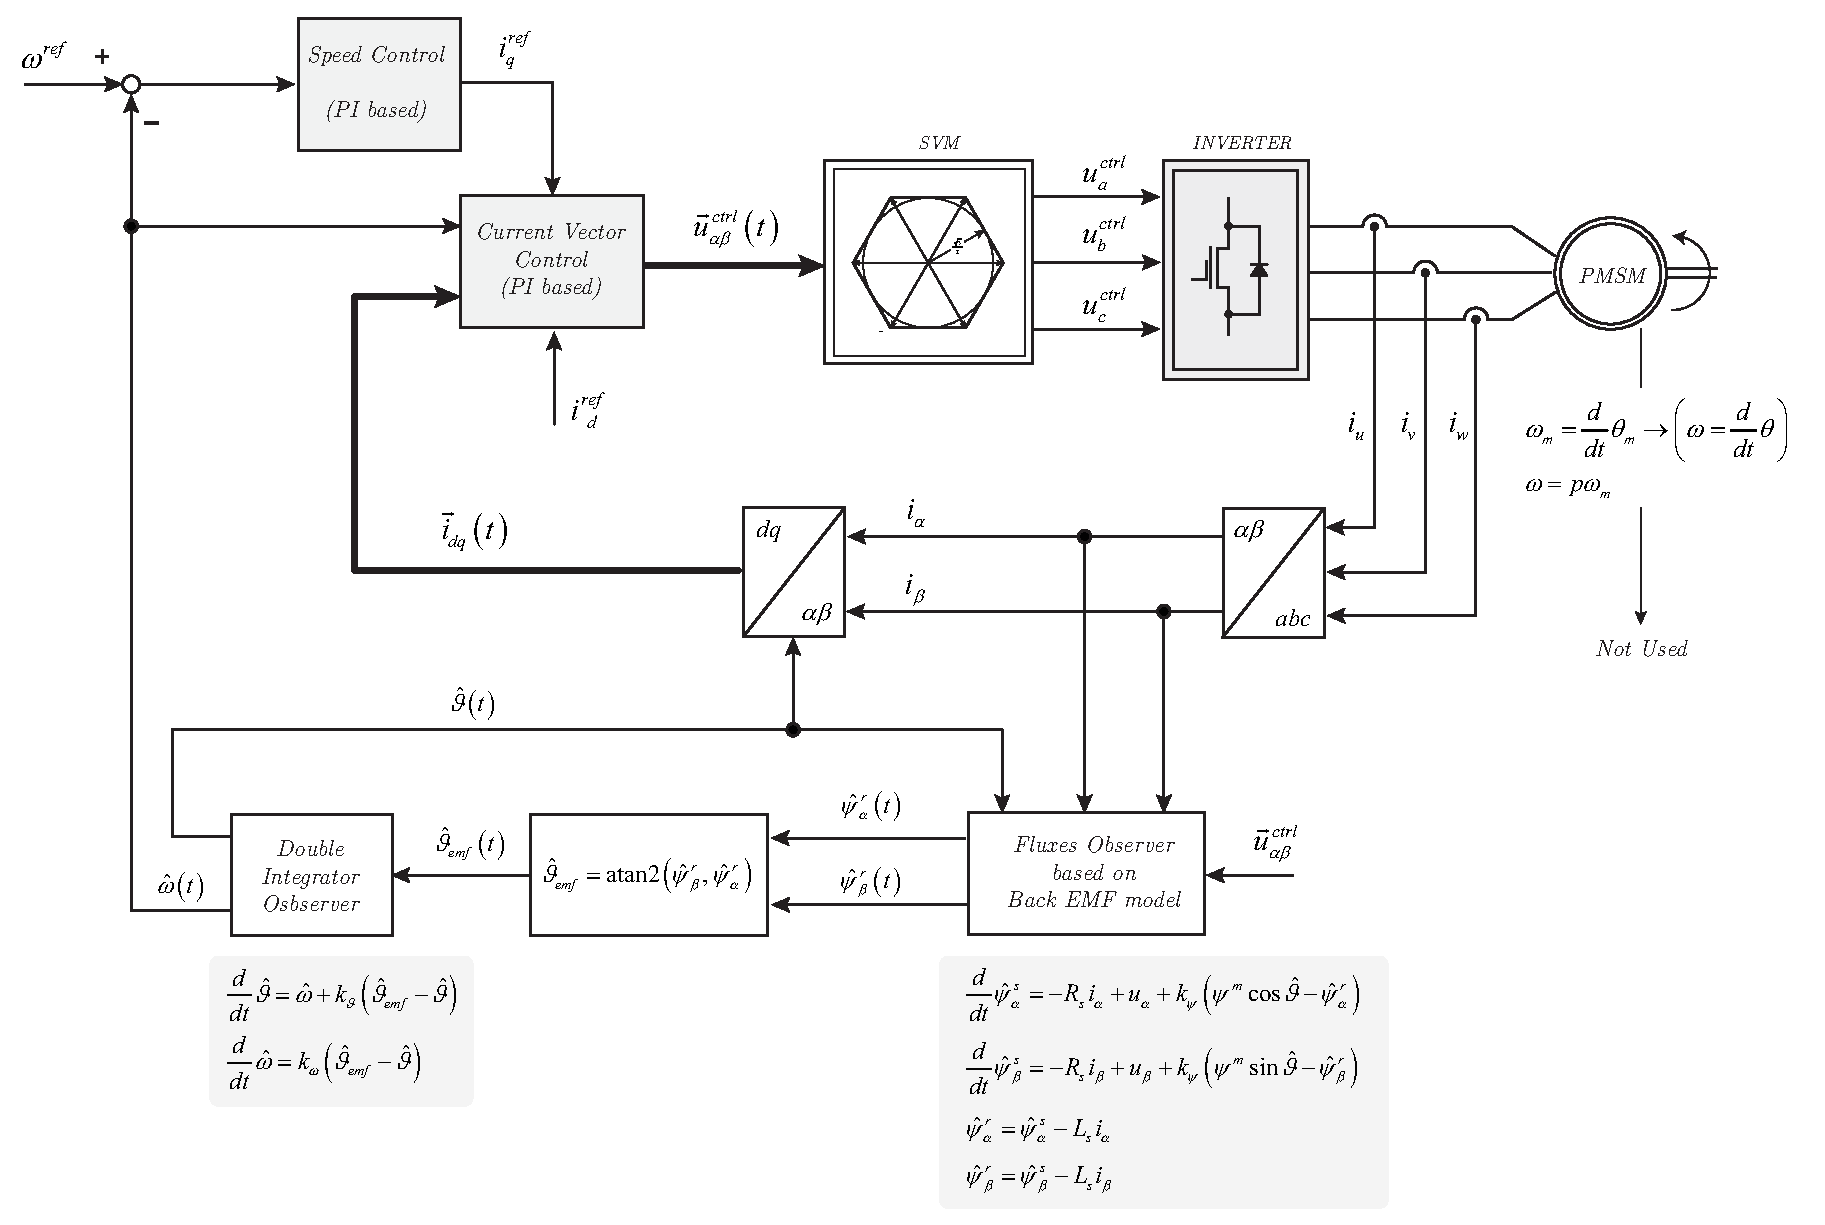
\includegraphics[height= 320pt, angle = 0, 
	keepaspectratio]{figures/control_layout/pmsm_sv_ctrl_scheme_1.eps}
	\captionsetup{width=0.5\textwidth, font=small}	
	\caption{State observer and vector control diagram.}
	\label{pmsm_sv_ctrl_scheme_1}
\end{figure}

\chapter{Firmware Implementation}
\section{Introduction}
In the following chapter the layout of the firmware implementation will be shown. The concept of the firmware implementation can be exploited as follows:
\begin{itemize}
	\item[--] device and peripherals configuration;
	\begin{itemize}
		\item[--] timer for the main task configuration ({\fontfamily{cmss}\selectfont \verb+TIM2+}) and synchronization with the timer for the three-phase PWM;
		\item[--] timer for the three-phase PWM with embedded dead-time configuration ({\fontfamily{cmss}\selectfont \verb+TIM1+}) and synchronization with the ADCs ({\fontfamily{cmss}\selectfont \verb+TRGO(2)+});
		\item[--] configuration of digital I/O ({\fontfamily{cmss}\selectfont \verb+GPIO+}) for \textit{mosfet} drivers enabling and over-current interrupts;
		\item[--] configuration of CANBUS communication;
	\end{itemize}
	\item[--] global software architecture which can be exploited as follows;
	\begin{itemize}
			\item[--] a main state machine process ({\fontfamily{cmss}\selectfont \verb+global_state_machine_process()+}) which coordinates the following sub-functions;
			\begin{itemize}
				\item[--] an automatic \textit{cmd} word generation ({\fontfamily{cmss}\selectfont \verb+global_cmd_word_generator_process()+}) which is triggered by the status of the \textit{can-bus} inputs and by the status of the \textit{DC-link} voltage power supply;
				\item[--] a sub-state-machine structure which properly selects the way of operation of the inverter control and triggers anomalous operating condition \\ ({\fontfamily{cmss}\selectfont \verb+inverter_state_machine_process()+});
				\item[--] the inverter inner controls are managed by a specific function which enables the inner vector current loops, state observers and operates the conversion from the machine state variables (\textit{uvw}) into the quadrature representation of the motor ($\alpha\beta$) and (\textit{dq}) ({\fontfamily{cmss}\selectfont \verb+inverter_ctrl_process()+});
			\end{itemize}
	\end{itemize}
	\item[--] additional ancillary and initialization functions have been implement as follows;
	\begin{itemize}
		\item[--] {\fontfamily{cmss}\selectfont \verb+peripherals_init()+}, where \text{DMA-ADC}, \text{IWD - independent watch-dog} and \text{DMA-PWM} have been initialized;
		\item[--] {\fontfamily{cmss}\selectfont \verb+adc_current_calibration()+};
		\item[--] {\fontfamily{cmss}\selectfont \verb+global_state_machine_init()+};
		\item[--] {\fontfamily{cmss}\selectfont \verb+global_cmd_word_generator_init()+};
		\item[--] {\fontfamily{cmss}\selectfont \verb+inverter_ctrl_init()+}.		
	\end{itemize}
\end{itemize}
\section{Device Configuration}
In this section the peripherals configuration of the STM32F746 is described. Conceptually a main task timer ({\fontfamily{cmss}\selectfont \verb+TIM2+}) is selected to generated a global interrupt which will be used for
	\begin{itemize}
	\item[--] start the main software process ({\fontfamily{cmss}\selectfont \verb+global_state_machine_process()+});
	\item[--] start and synchronize the PWM timer ({\fontfamily{cmss}\selectfont \verb+TIM1+}).		
\end{itemize}
Analog acquisition are automatically activated by the signal ({\fontfamily{cmss}\selectfont \verb+TRGO(2)+}) regularly launched by the ({\fontfamily{cmss}\selectfont \verb+TIM1+}) at every vertex of the PWM carry triangle waveform (this is activated by selecting {\fontfamily{cmss}\selectfont \verb+Repetition Counter = 0+}).
The overall timing of the ({\fontfamily{cmss}\selectfont \verb+TIM2+}) and ({\fontfamily{cmss}\selectfont \verb+TIM1+}) can be seen as depicted in Figure~\ref{adc_synch}.
\begin{figure}[H]
	\centering
	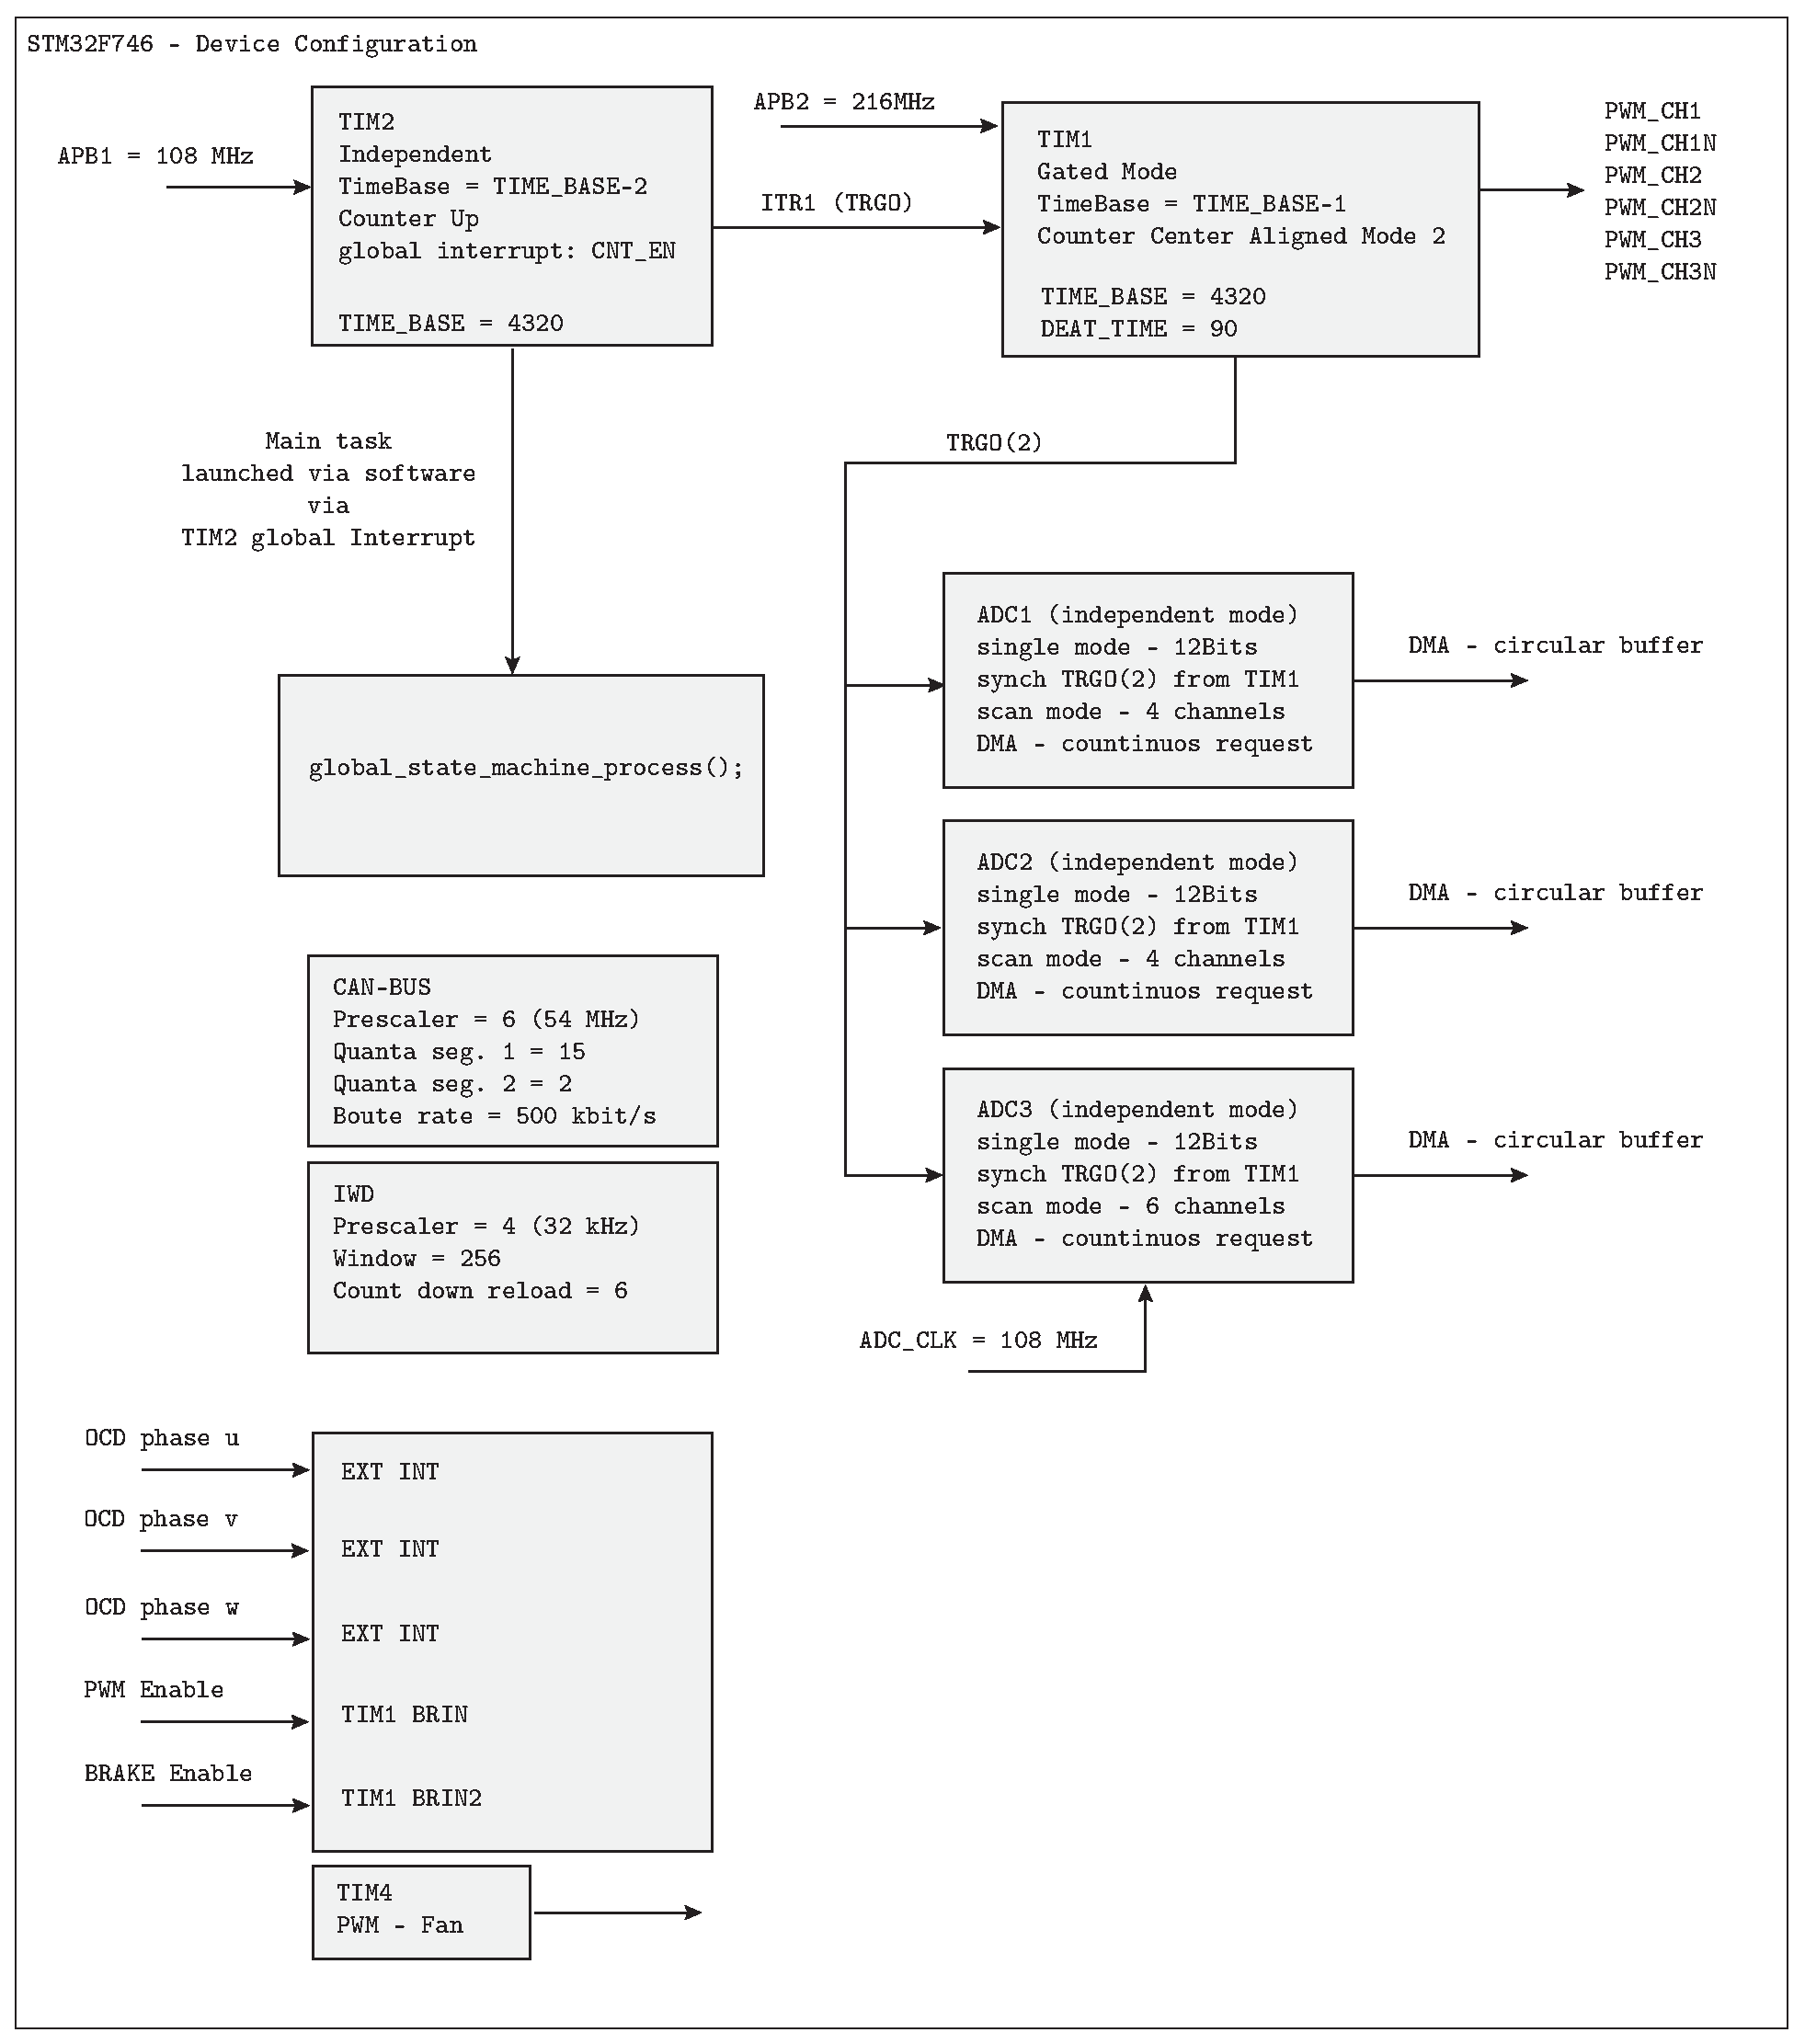
\includegraphics[width= 475pt, angle = 0, 
	keepaspectratio]{figures/firmware_arch/device_config_1.eps}
	\captionsetup{width=0.5\textwidth, font=small}	
	\caption{Device configuration overview.}
	\label{device_config_1}
\end{figure}

\begin{figure}[H]
	\centering
	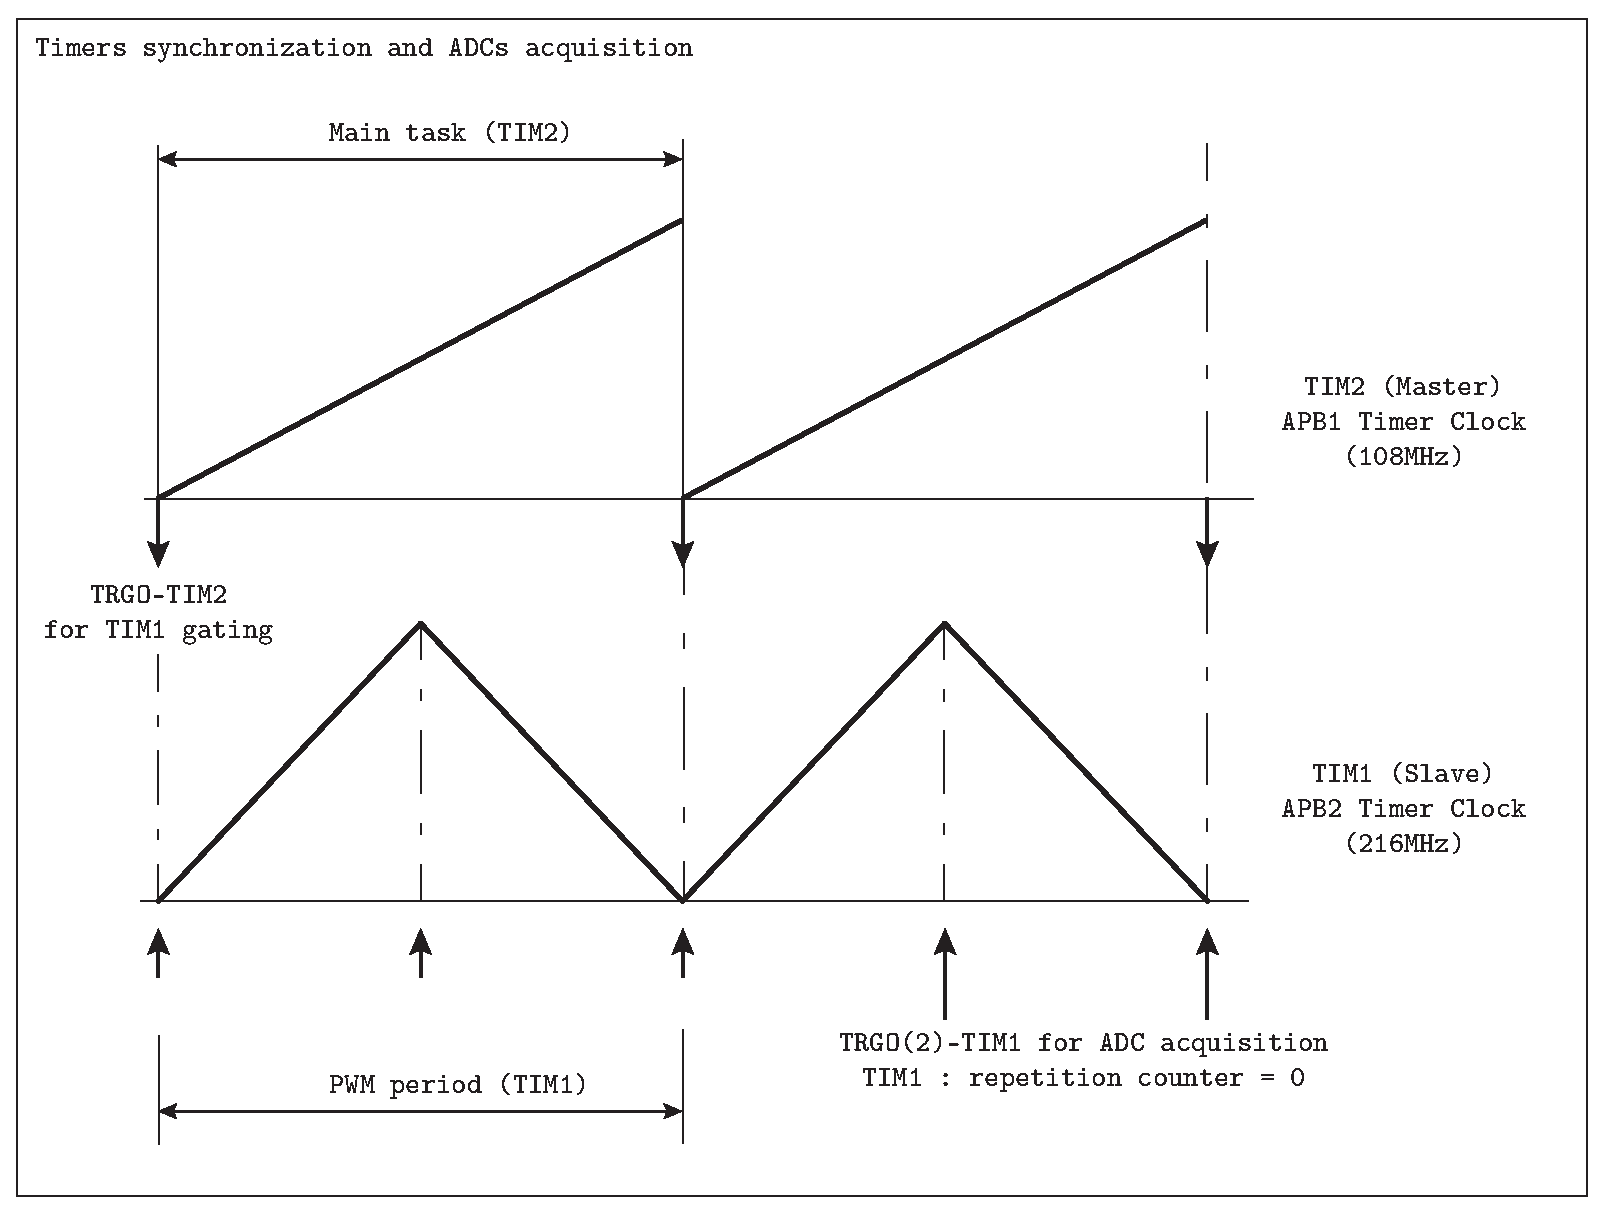
\includegraphics[height= 300pt, angle = 0, 
	keepaspectratio]{figures/firmware_arch/adc_synch.eps}
	\captionsetup{width=0.5\textwidth, font=small}	
	\caption{ADCs and PWM synchronization overview.}
	\label{adc_synch}
\end{figure}

\section{State Machines and control architecture}
The global control application is based on two main state machine control 
\begin{itemize}
	\item[--] {\fontfamily{cmss}\selectfont \verb+global_state_machine_process()+};
	\item[--] {\fontfamily{cmss}\selectfont \verb+inverter_state_machine_process()+};
\end{itemize}
these states machines coordinates the status of a \textit{global system} with the status of a \textit{inner system}. The \textit{inner system} manages the {\fontfamily{cmss}\selectfont \verb+inverter_control_process()+}, see Figure~\ref{software_architecture}; 
\begin{figure}[H]
	\centering
	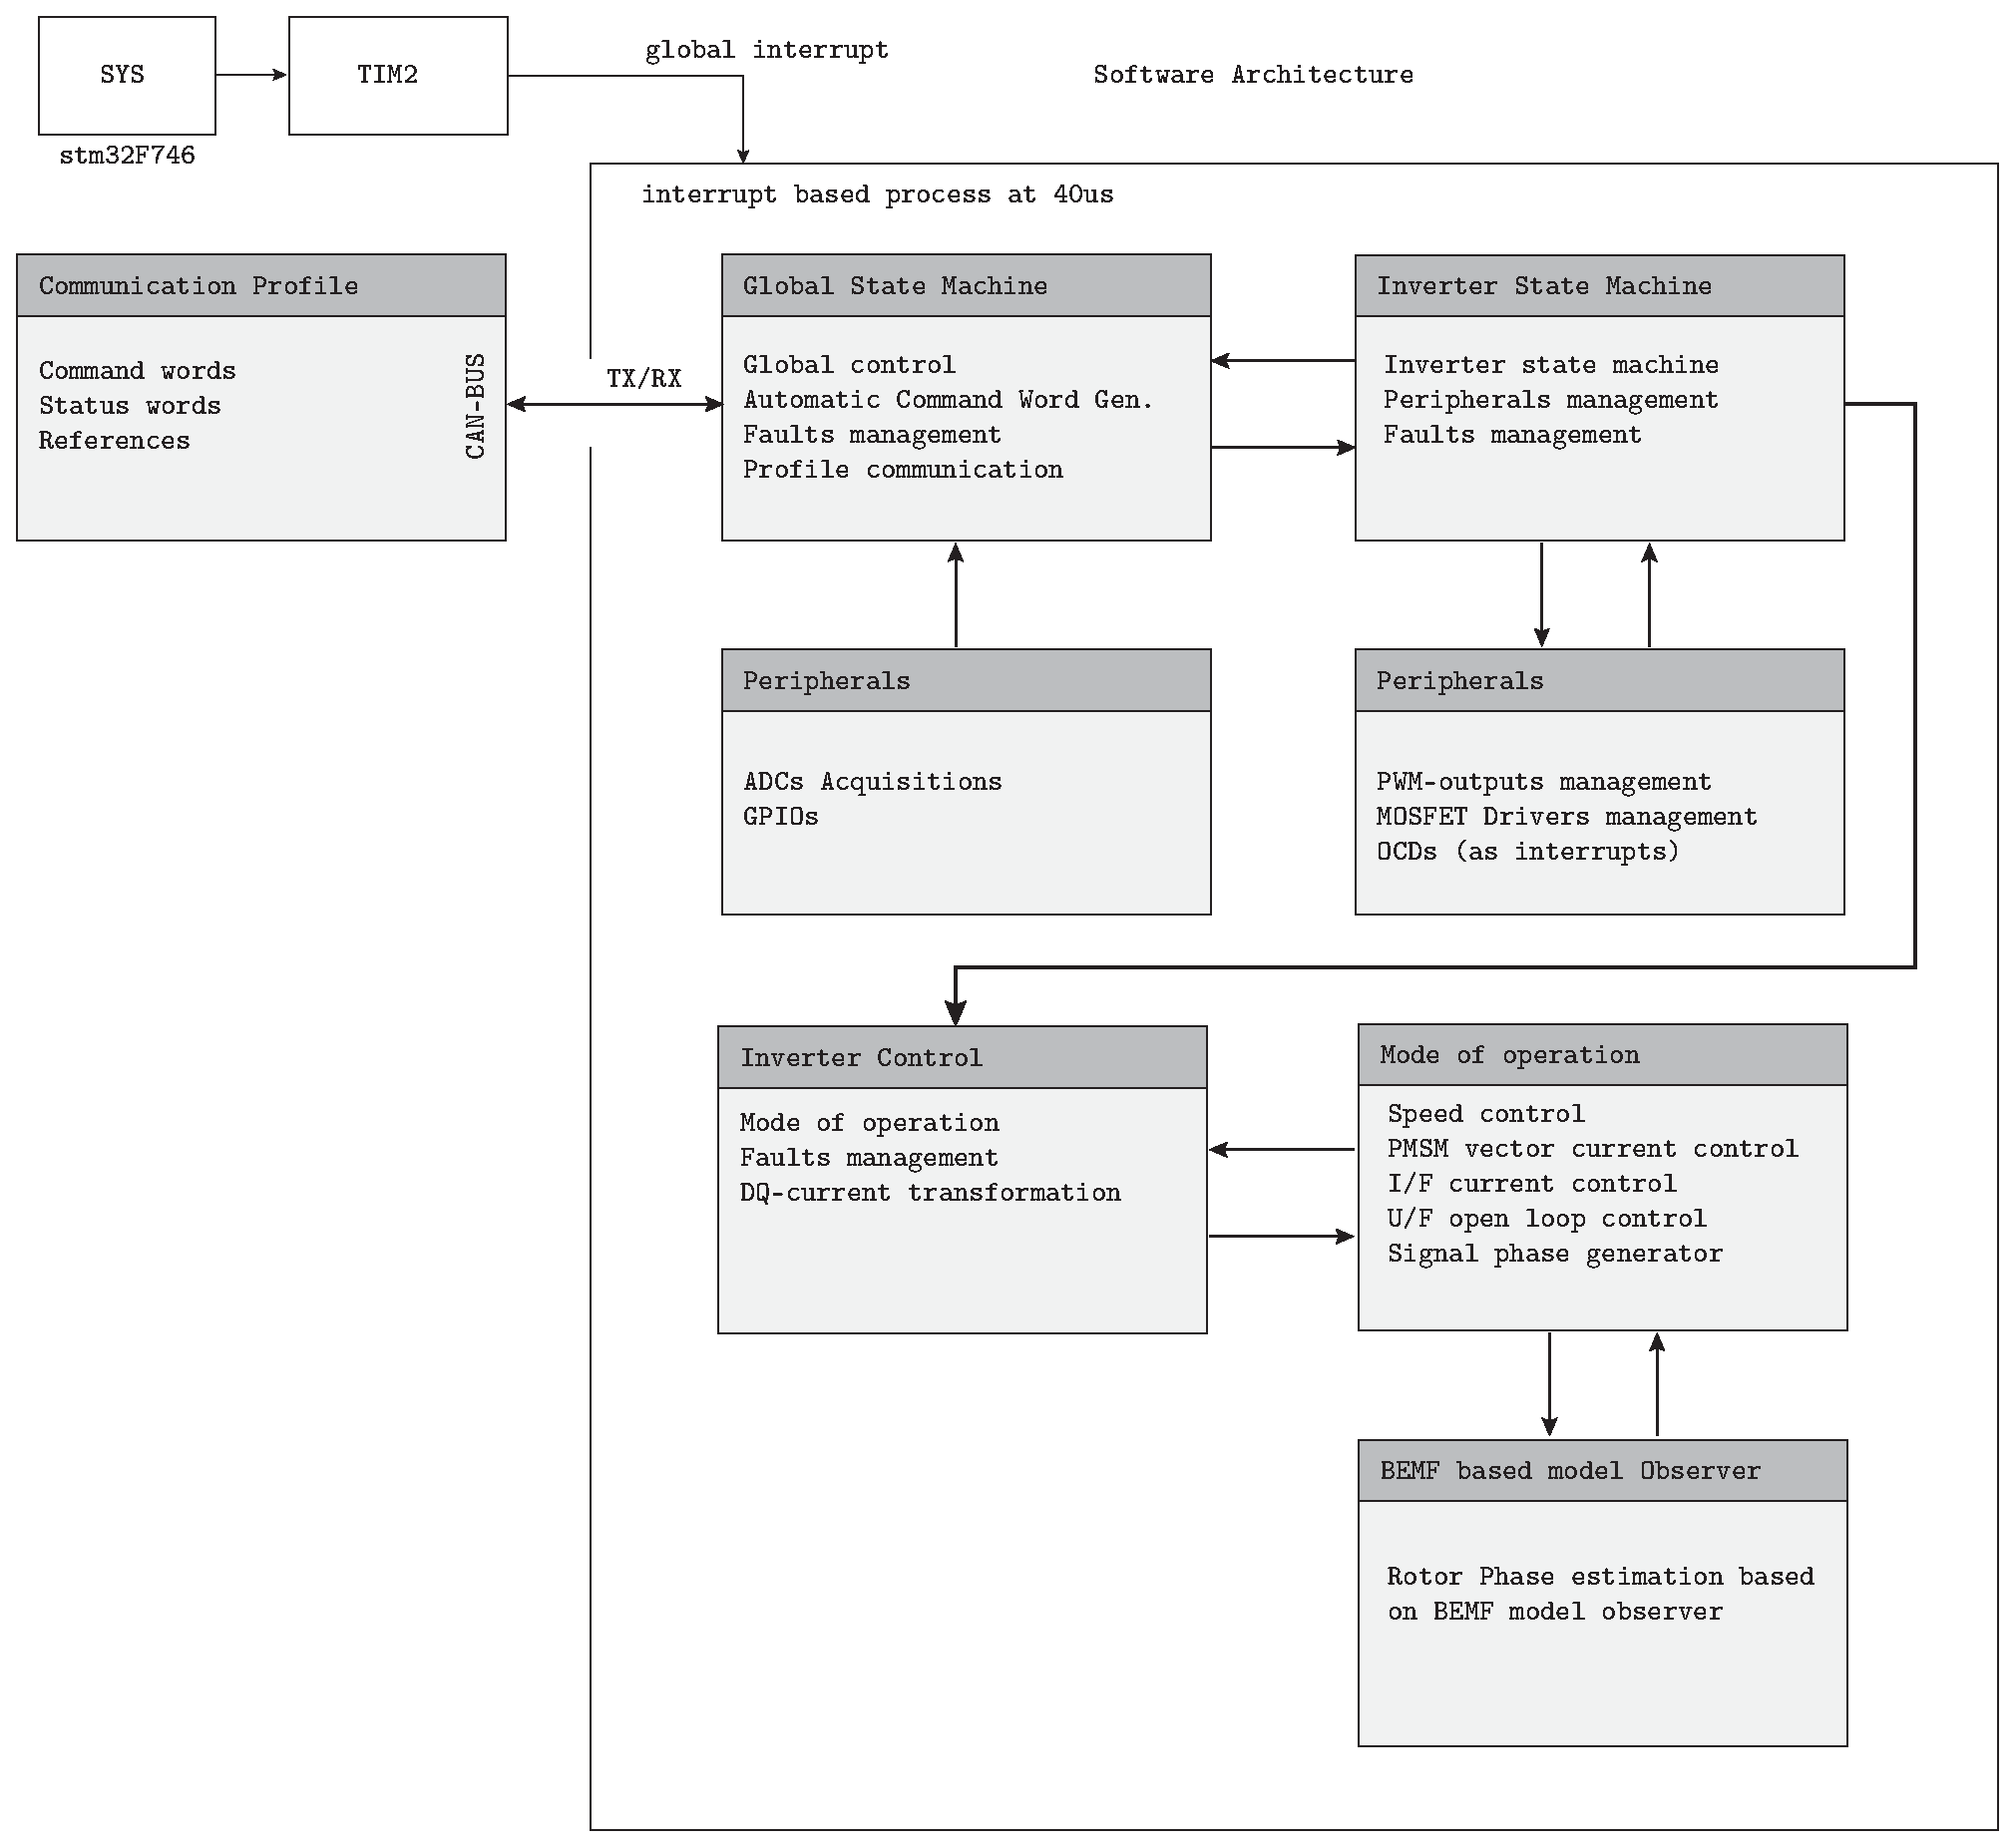
\includegraphics[width = 475pt, angle = 0, 
	keepaspectratio]{figures/firmware_arch/software_architecture_2.eps}
	\captionsetup{width=0.5\textwidth, font=small}	
	\caption{Global state machine and auxiliary functions architecture overview.}
	\label{software_architecture}
\end{figure}
Figure~\ref{global_state_machine} shows a qualitative representation the state machine flow of the \\ {\fontfamily{cmss}\selectfont \verb+global_state_machine_process()+}.
\begin{figure}[H]
	\centering
	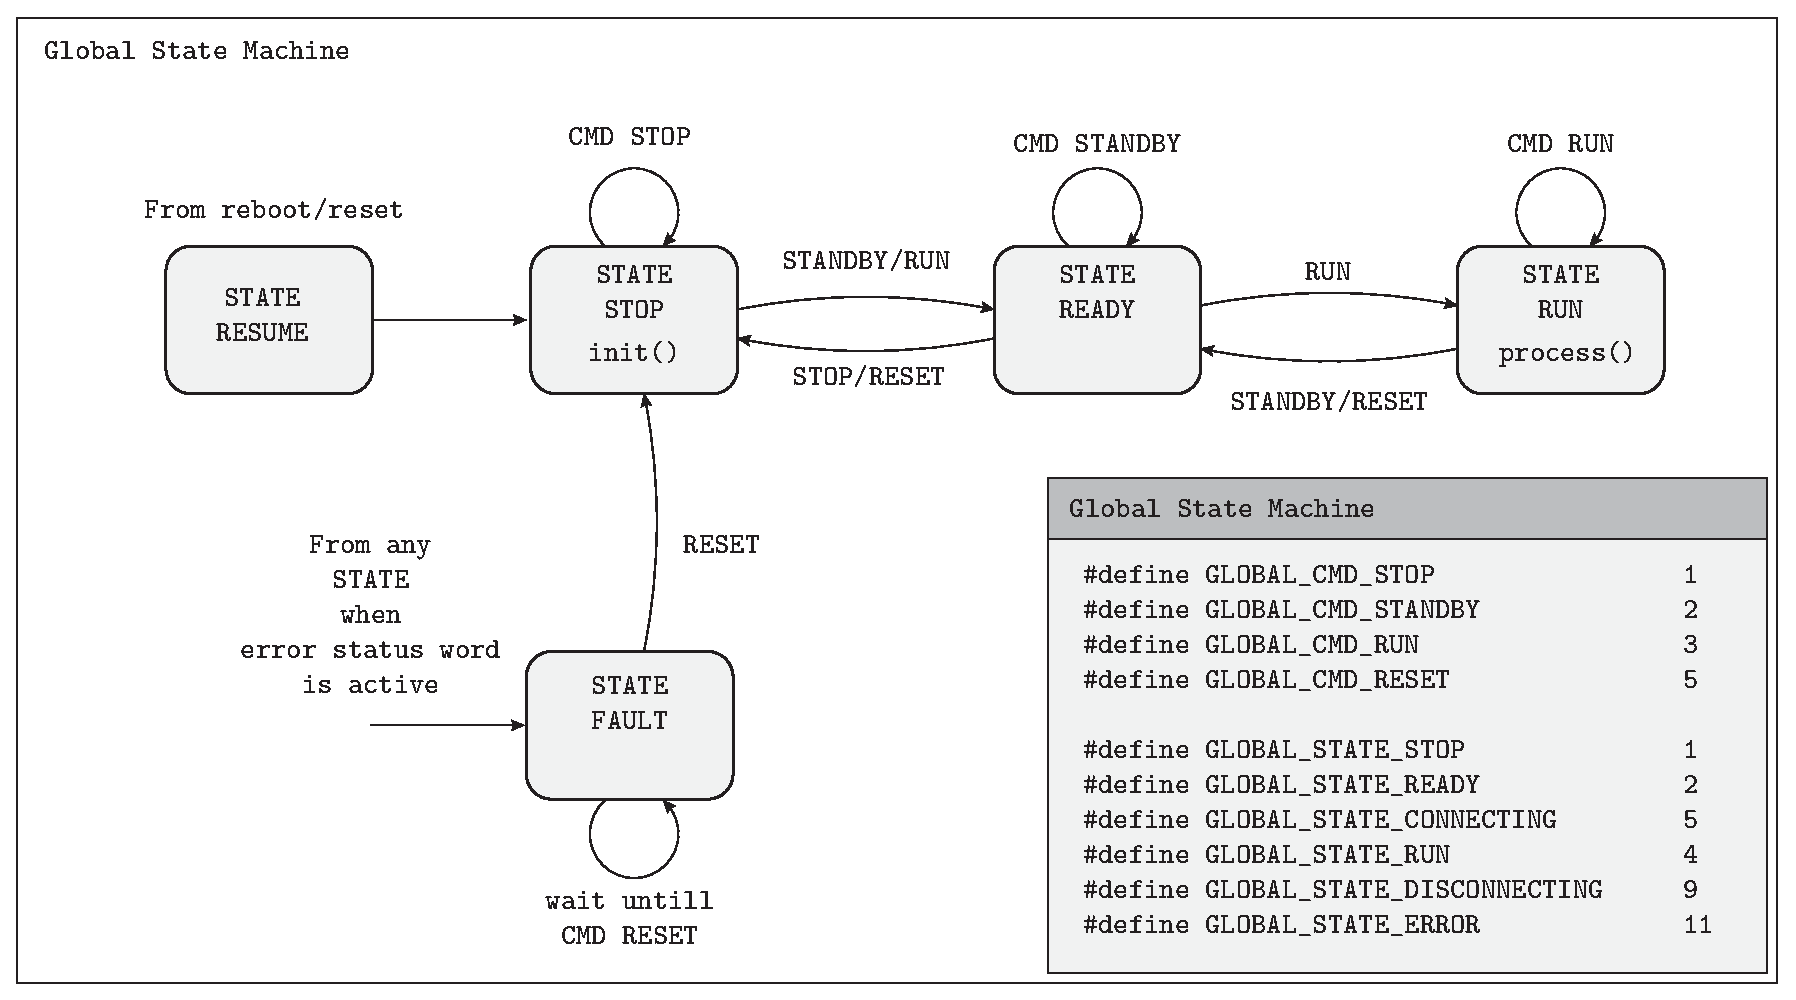
\includegraphics[height= 260pt, angle = 0, 
	keepaspectratio]{figures/firmware_arch/global_state_machine.eps}
	\captionsetup{width=0.5\textwidth, font=small}	
	\caption{Global state machine overview.}
	\label{global_state_machine}
\end{figure}
Figure~\ref{inverter_state_machine} shows a qualitative representation the state machine flow of the \\ {\fontfamily{cmss}\selectfont \verb+inverter_state_machine_process()+}.
\begin{figure}[H]
	\centering
	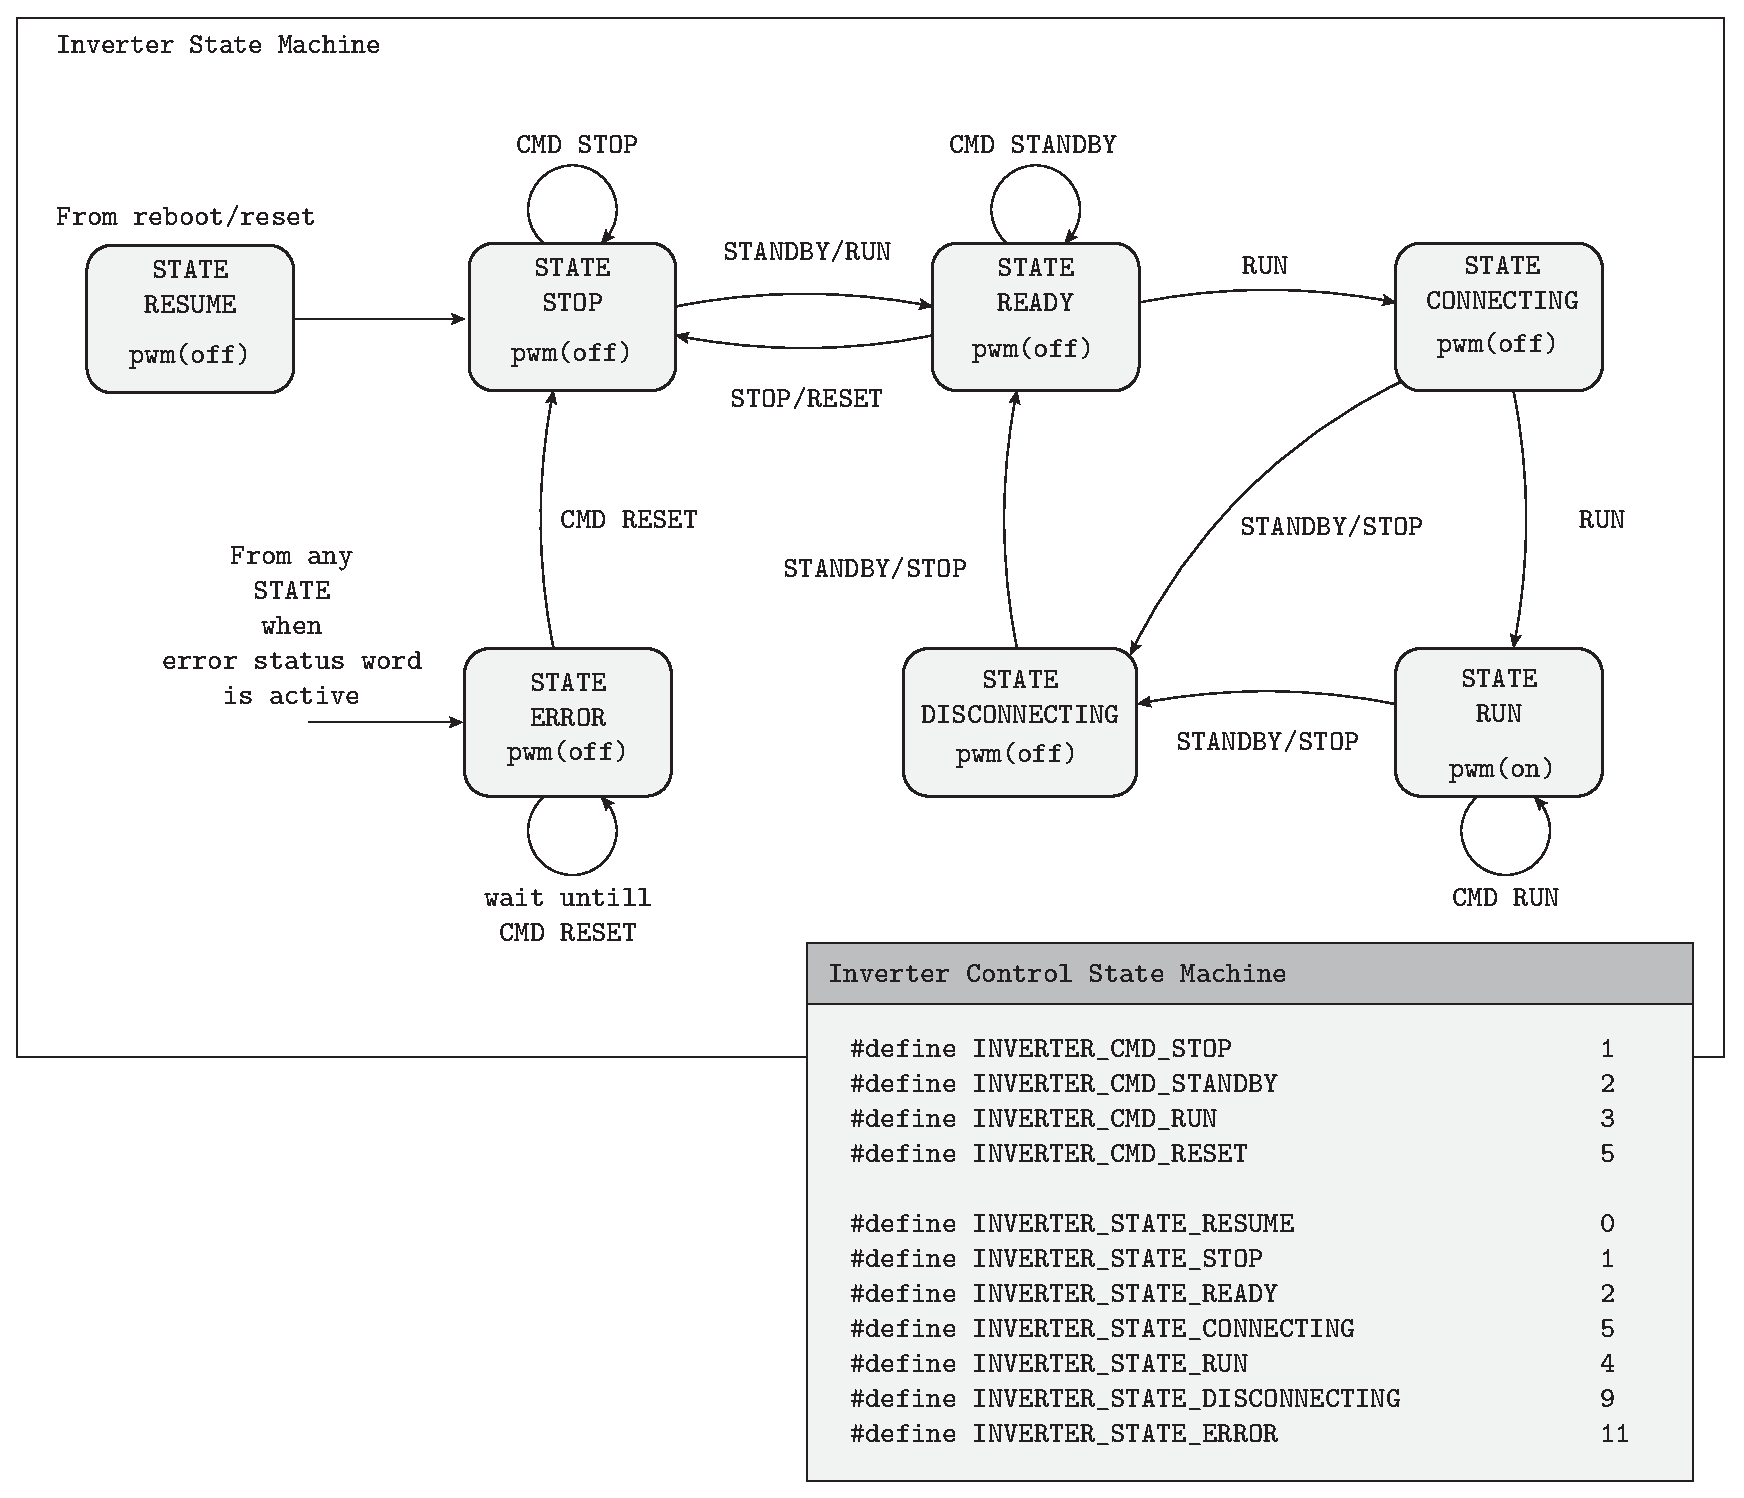
\includegraphics[height= 400pt, angle = 0, 
	keepaspectratio]{figures/firmware_arch/inverter_state_machine.eps}
	\captionsetup{width=0.5\textwidth, font=small}	
	\caption{Inverter state machine overview.}
	\label{inverter_state_machine}
\end{figure}

An additional software control block concerns the automatic generation of the command word for the \\ {\fontfamily{cmss}\selectfont \verb+global_state_machine_process()+}.  
Figure~\ref{global_cmd_word_generator_process} shows the implemented solution, which can be summarized as follows:
\begin{itemize}
	\item[--] The DC-link voltage measure is filtered and sent to a comparator for unconstrained {\fontfamily{cmss}\selectfont \verb+STANDBY/STOP+} internal commands;
	\item[--] The duty reference word received from can bus is filtered and sent to a comparator for constrained {\fontfamily{cmss}\selectfont \verb+RUN/STANDBY+} internal commands;	
\end{itemize}
Figure~\ref{global_cmd_word_generator_state_machine} shows the internal state machine of the {\fontfamily{cmss}\selectfont \verb+global_state_machine_process()+}.
\begin{figure}[H]
	\centering
	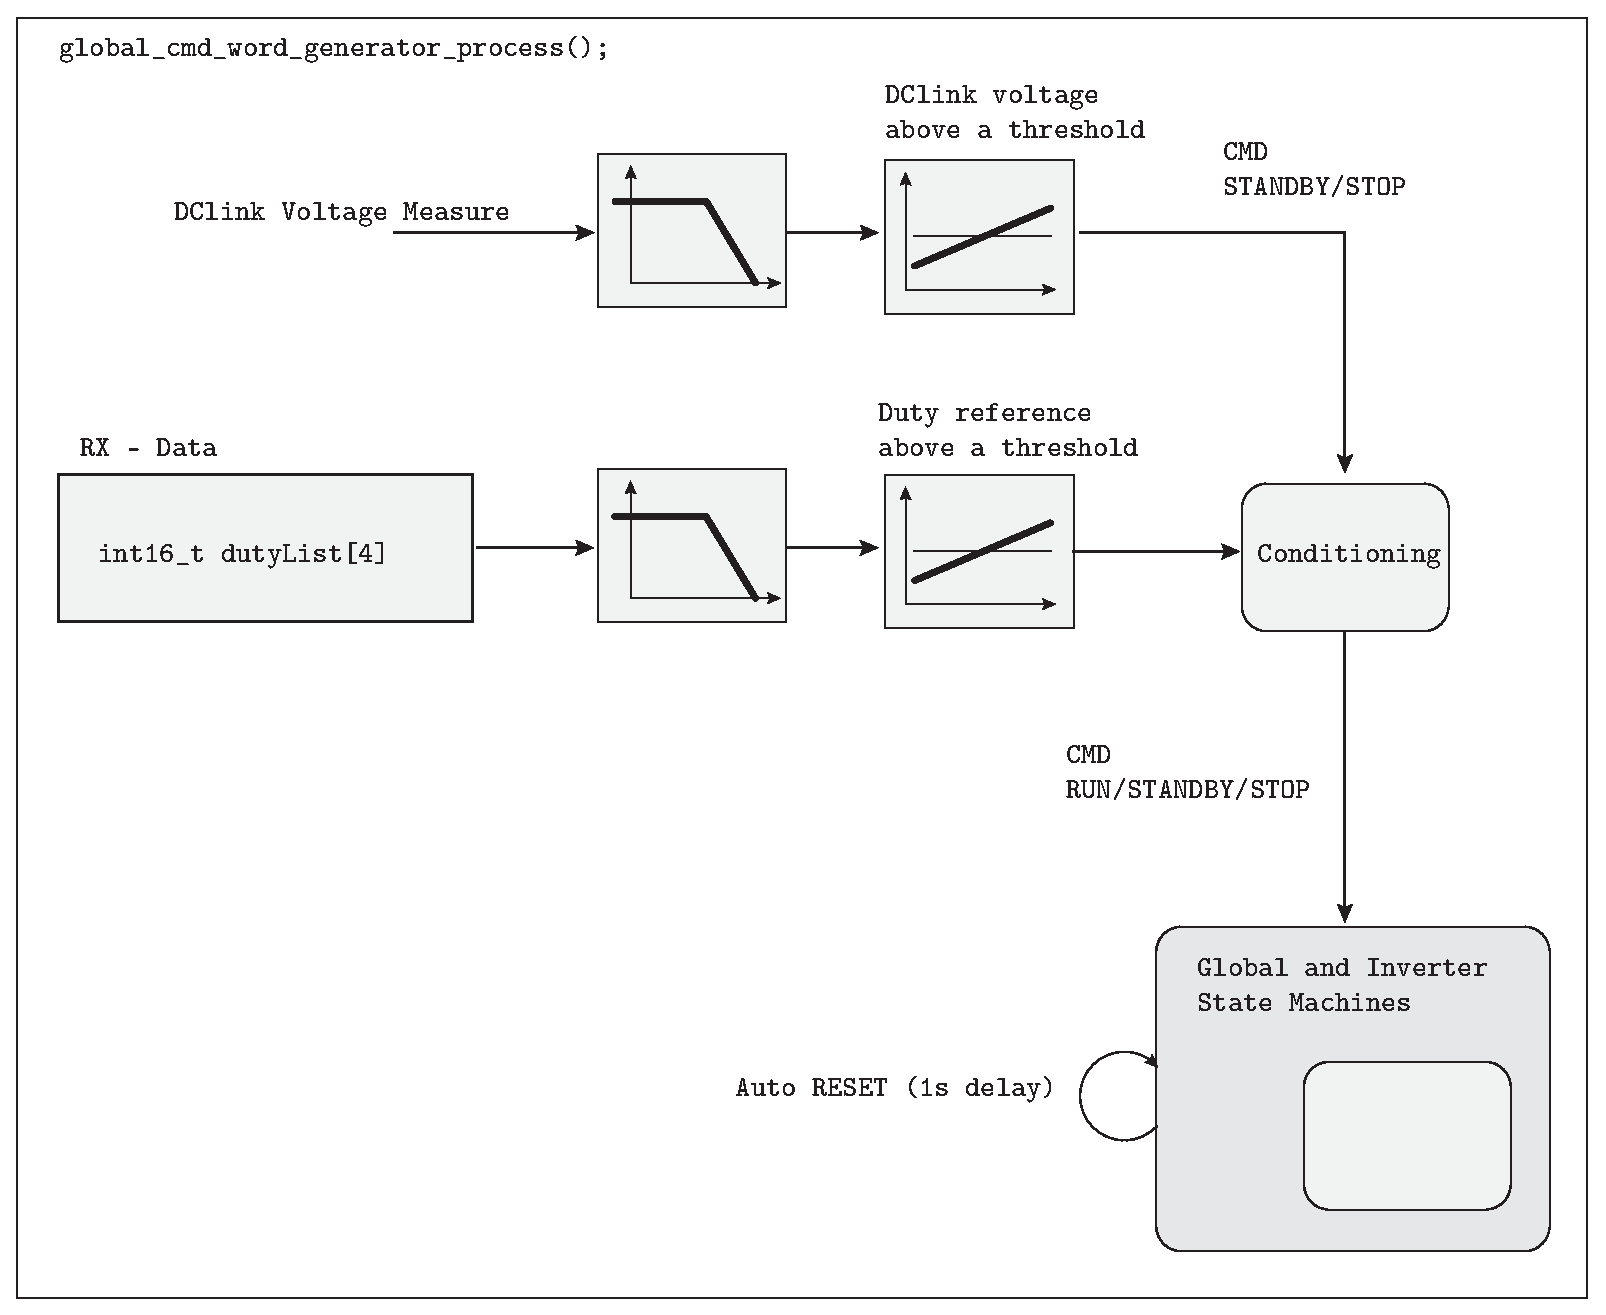
\includegraphics[width= 450pt, angle = 0, 
	keepaspectratio]{figures/firmware_arch/global_cmd_word_generator_process.eps}
	\captionsetup{width=0.5\textwidth, font=small}	
	\caption{Automatic command word generation overview.}
	\label{global_cmd_word_generator_process}
\end{figure}
\begin{figure}[H]
	\centering
	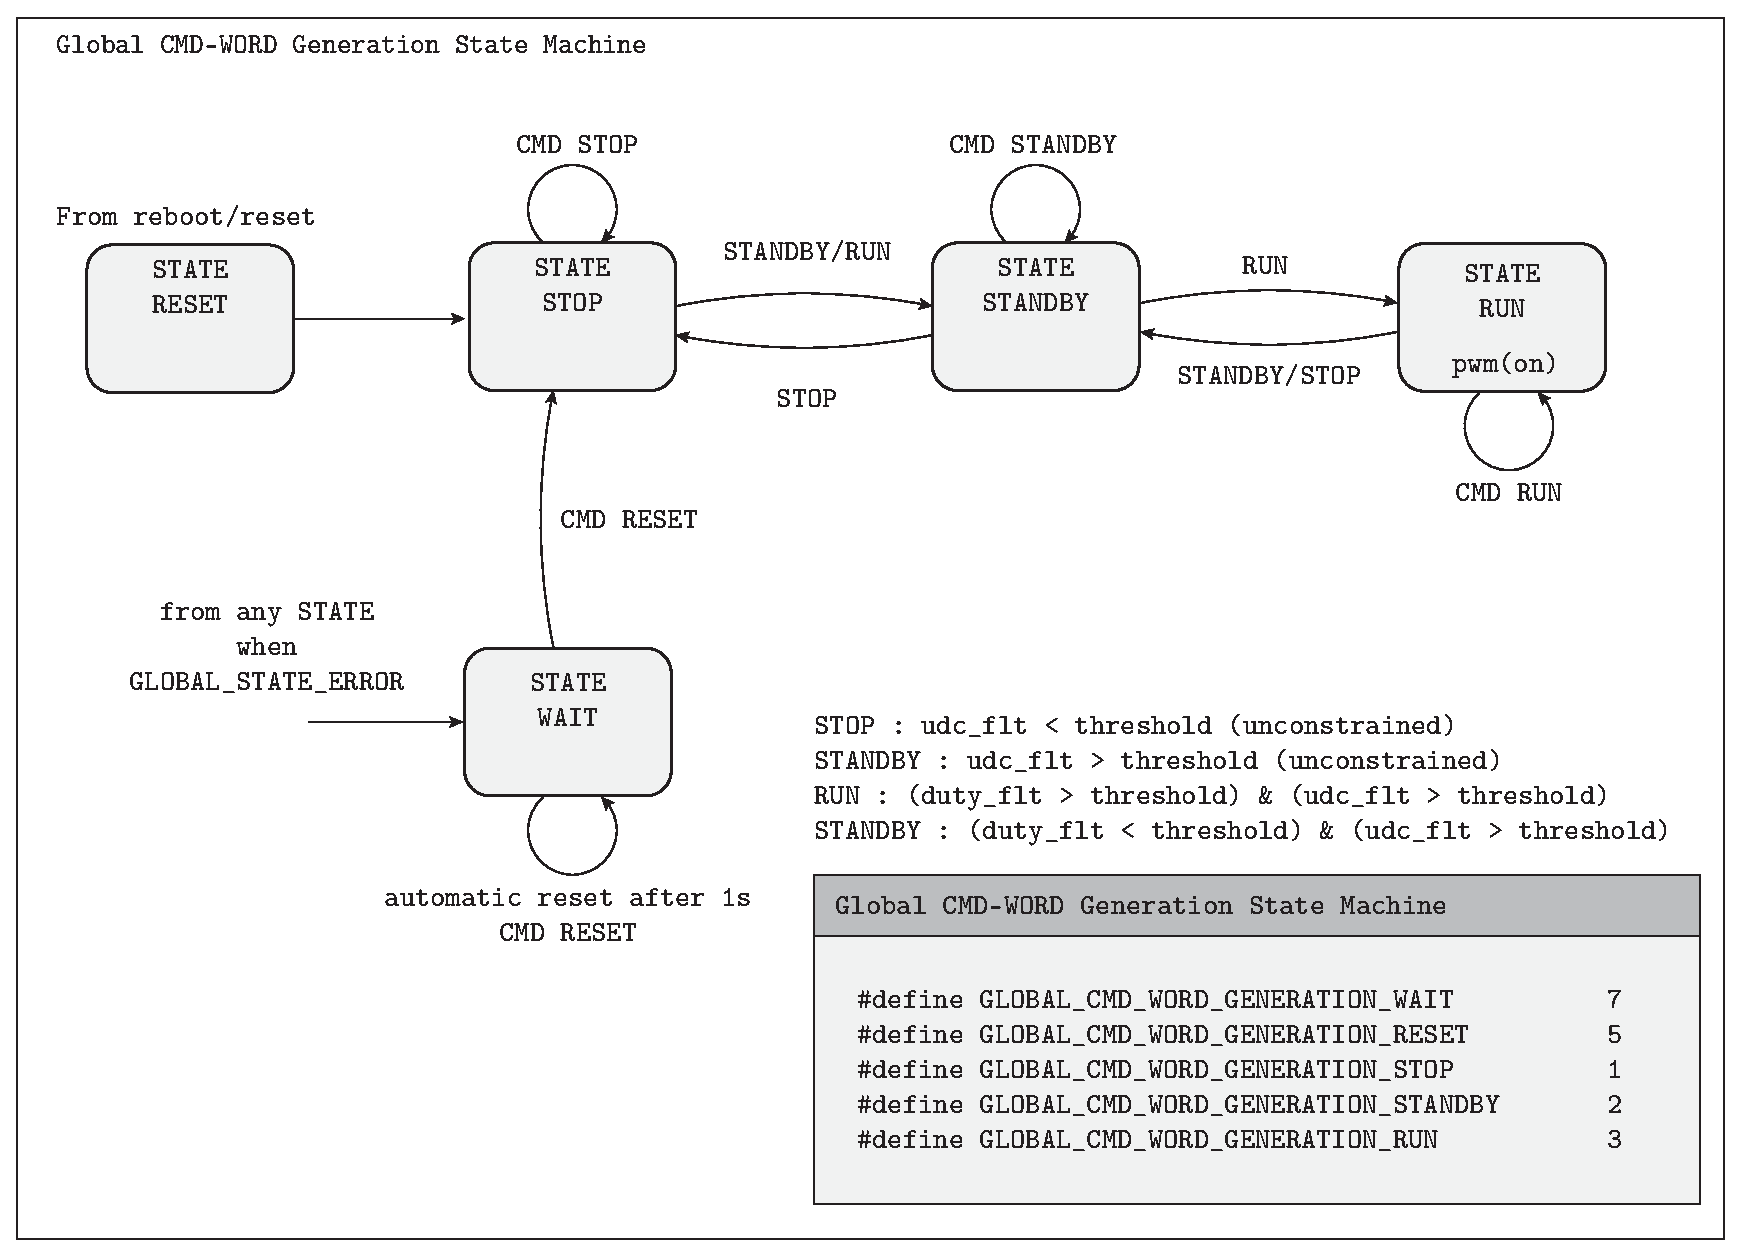
\includegraphics[width= 450pt, angle = 0, 
	keepaspectratio]{figures/firmware_arch/global_cmd_word_generator_state_machine.eps}
	\captionsetup{width=0.5\textwidth, font=small}	
	\caption{Automatic command word generation state machine.}
	\label{global_cmd_word_generator_state_machine}
\end{figure}

\chapter{Appendix A - Control Engineering}
\section{State Observer}\label{state_observer_theory} 
In the pole placement approach the design of a control system assumes that 
all state variable are available for feedback. In practice, however, not all 
state variables are available for feedback. That, the need to estimate 
unavailable state variables using the theory of the \textit{state observer} or \textit{Luenberger observer}.

\vspace{5mm}
\textbf{Luenberger observer}. A state observer estimates the state variables based 
on the measurements of the output and control variables. \textit{State 
	observers can be designed if and only if the observability condition is 
	satisfied.}
Considering the plant defined by
\begin{equation} \label{state_observer_1}
	\begin{split}
		\dot{\vec x} & = \tilde{\mathbf{A}}\vec{x} + \tilde{\mathbf{B}}u \\[6pt]
		y & = \mathbf{C}\vec{x}
	\end{split}
\end{equation}
The observer is a subsystem to reconstruct the state vector of the plant. The 
mathematical model of the observer is basically the same as that of the plant, 
except that we include an additional term that includes the estimation error to 
compensate for inaccuracies in matrices $\tilde{\mathbf{A}}$ and 
$\tilde{\mathbf{B}}$ and the lack of the initial error.The estimation error or 
the observation error is the difference between the measured output and the 
estimated output. The initial error is the difference between the initial state 
and the initial estimated state. Thus, we define the mathematical model of the 
observer to be
\begin{equation} \label{state_observer_2}
	\begin{split}
		\dot{\hat{\vec{x}}} & = \tilde{\mathbf{A}}\hat{\vec x} + 
		\tilde{\mathbf{B}}\vec u + \mathbf{L}(y - \mathbf{C}\hat{\vec x}) 
		\\
		& = (\tilde{\mathbf{A}}-\mathbf{L}\mathbf{C})\hat{\vec x} + 
		\tilde{\mathbf{B}}u + \mathbf{L}y
	\end{split}
\end{equation}
where $\hat{\vec x}$ is the estimated state and $\mathbf{C}\hat{\vec x}$ is the 
estimated output. \textit{The inputs of the observer are the output $\vec y$ 
	and the control input $\vec u$}. Matrix $\mathbf{L}$ which is called the 
observer gain matrix, is a weighting matrix to the correction term involving 
the difference between the measured output $\vec y$ and the estimated output 
$\mathbf{C}\hat{\vec x}$. this term continuously corrects the model output and 
improves 
the performance of the observer. Figure~\ref{figure_state_observer} shows the 
block diagram of the system and the full-order state observer.
The order of the state observer that will be discussed here is the same as that 
of the plant.

To obtain the observer error equation, let us subtract 
Eq.~\eqref{state_observer_2} from 
Eq.~\eqref{state_observer_1}:
\begin{equation} \label{state_observer_3}
	\begin{split}
		\dot{\vec{x}} - \dot{\hat{\vec x}} & = \tilde{\mathbf{A}}\vec x - 
		\tilde{\mathbf{A}}\hat{\vec x} - \mathbf{L}(\mathbf{C}\vec x - 
		\mathbf{C}\hat{\vec{x}}) \\
		& = (\mathbf{\mathbf{A}}-\mathbf{L}\mathbf{C})(\vec{x} - \hat{\vec{x}})
	\end{split}
\end{equation}
Define the difference between $\vec{x}$ and $\hat{\vec{x}}$ as the error vector 
$\vec{e}$, or
\begin{equation} \label{state_observer_4}
	\vec{e} = \vec{x} - \hat{\vec{x}}
\end{equation}
the equation (\ref{state_observer_3}) becomes
\begin{equation} \label{state_observer_5}
	\dot{\vec{e}} = (\tilde{\mathbf{A}}-\mathbf{LC})\vec{e}
\end{equation}
From Eq.~\eqref{state_observer_5}, we see that the dynamic behaviour of the 
error vector is 
determined by the eigenvalues of matrix $(\tilde{\mathbf{A}}-\mathbf{LC})$. If 
matrix $(\tilde{\mathbf{A}}-\mathbf{LC})$ is a stable matrix, the error vector 
will converge to zero for any initial error vector $\vec e(0)$. That is, 
$\hat{\vec x}(t)$ will 
converge to $\vec x(t)$ regardless of the value of $\vec x(0)$ and 
$\hat{\vec{x}}(0)$. If the eigenvalues of the matrix 
$(\tilde{\mathbf{A}}-\mathbf{LC})$ are chosen in such a way that the dynamic 
behaviour of the error vector is asymptotically stable and is adequately fast, 
then any error vector will tend to zero (the origin) with an adequate speed.
If the plant is completely observable, then it can be proved that it is 
possible to choose matrix $\mathbf{L}$ such that 
$(\tilde{\mathbf{A}}-\mathbf{LC})$ has 
arbitrarily desired eigenvalues. That is, the observer gain matrix $\mathbf{L}$ 
can be determined to yield the desired matrix 
$(\tilde{\mathbf{A}}-\mathbf{LC})$. 
\begin{figure}[H]
	\centering
	\begin{subfigure}{.75\textwidth}
		\centering
		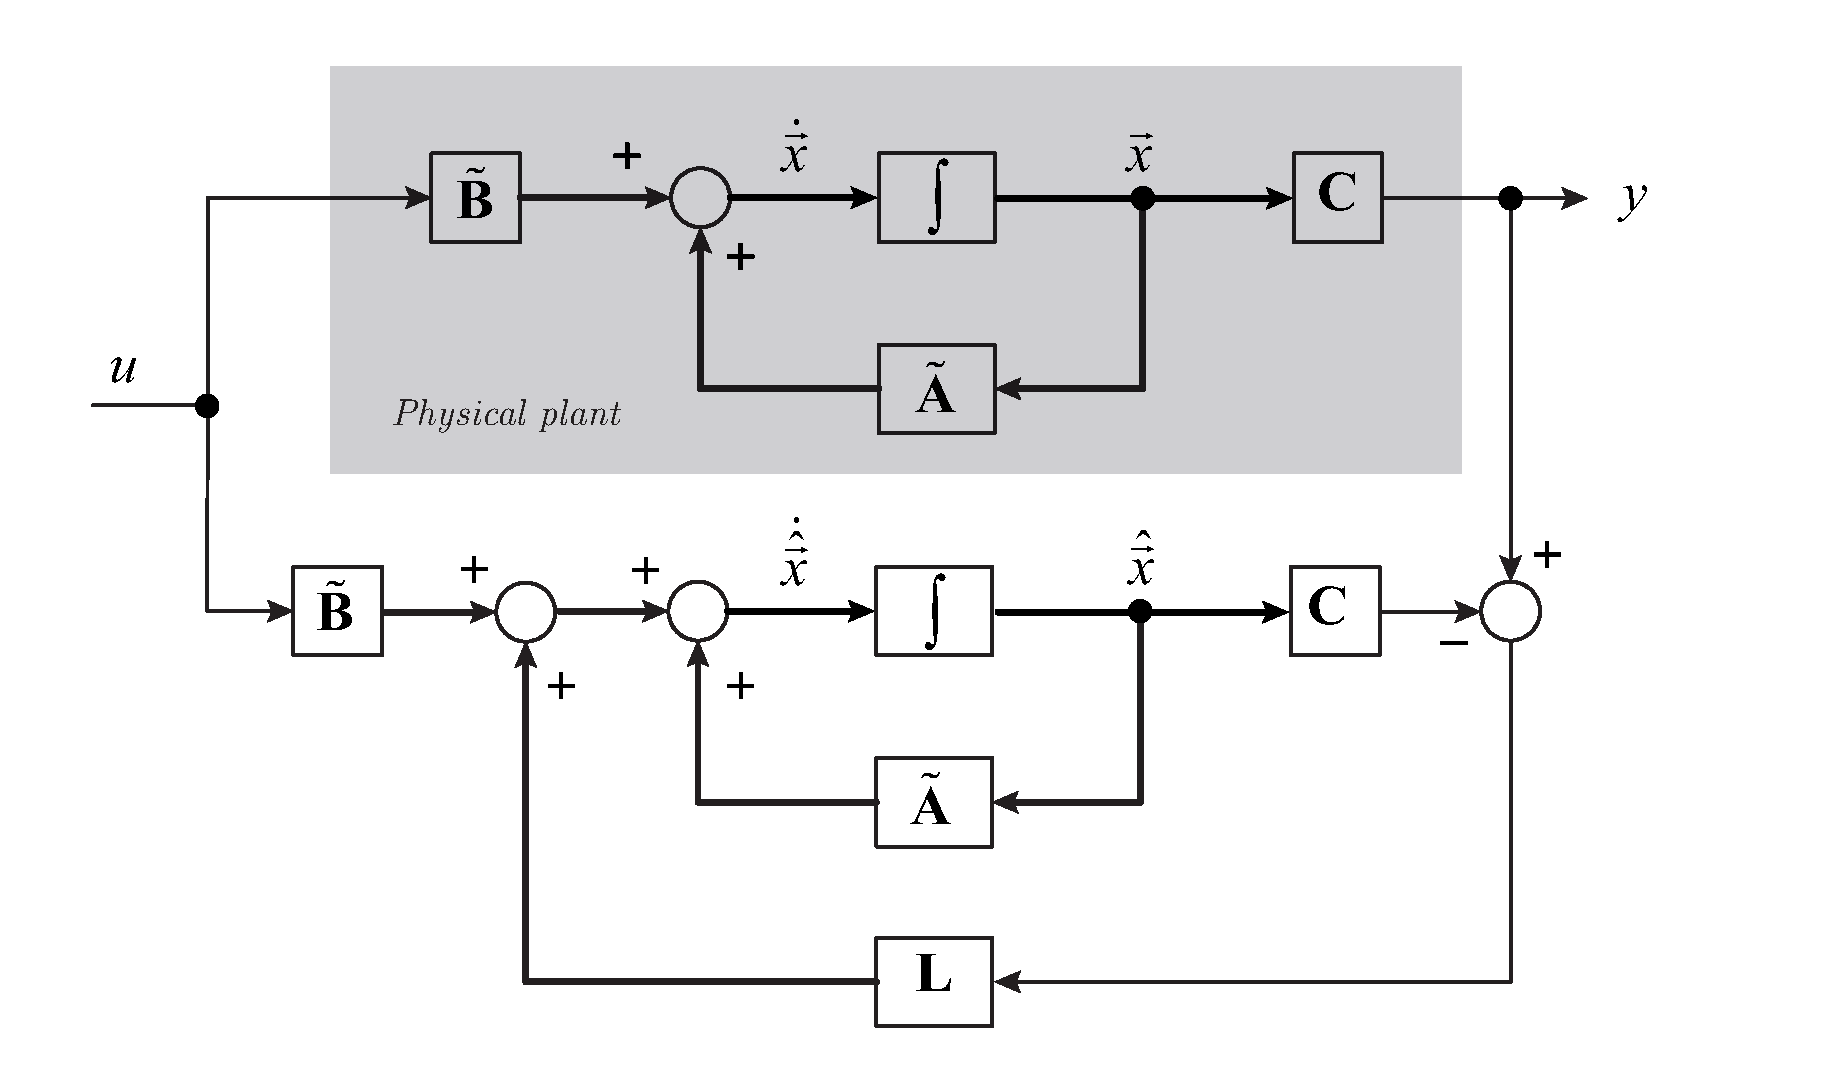
\includegraphics[width = 340pt, 
		keepaspectratio]{figures/state_observer_1.eps}
		\captionsetup{width = 0.5\textwidth, font=footnotesize}
		\caption{Physical Plant in the form of state space representation.}
		\label{figure_state_observer1}
	\end{subfigure}	
	\begin{subfigure}{.75\textwidth}
		\centering
		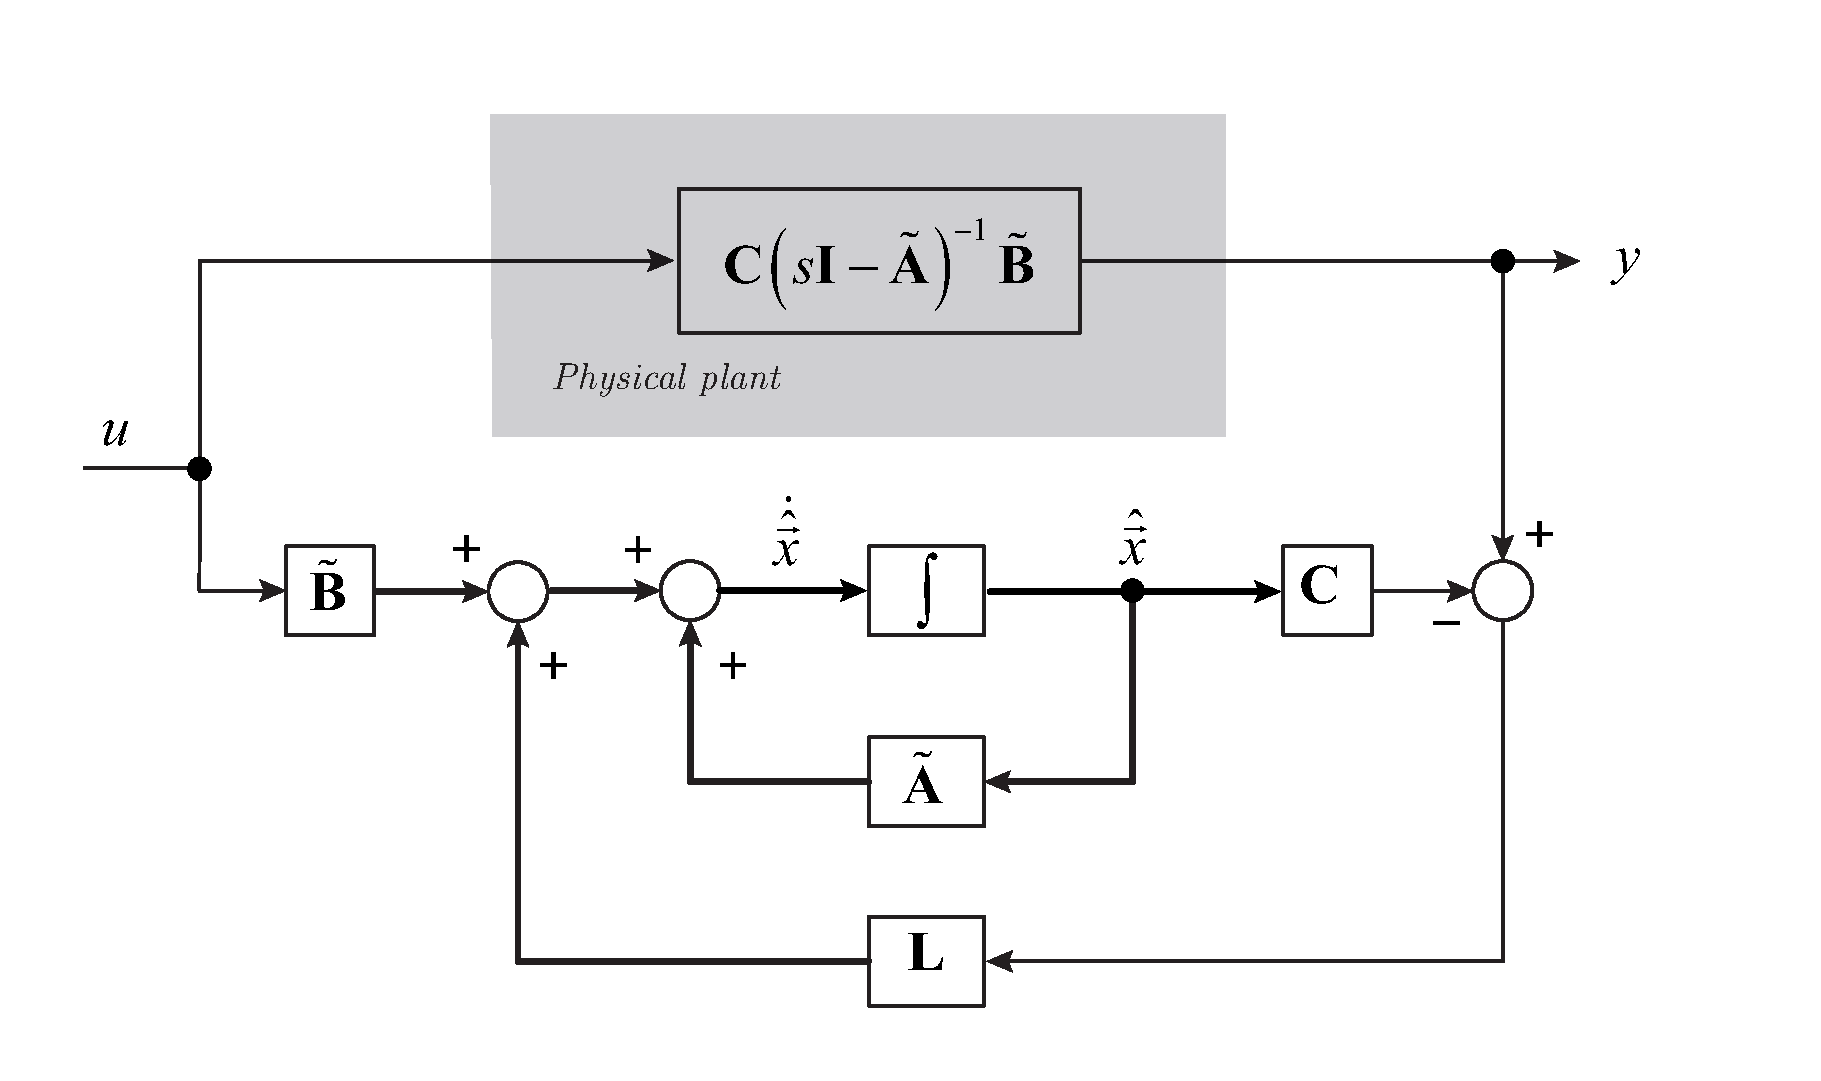
\includegraphics[width = 340pt, 
		keepaspectratio]{figures/state_observer_2.eps}
		\captionsetup{width = 0.5\textwidth,font=footnotesize}
		\caption{Physical Plant in the form of transfer function.}
		\label{figure_state_observer2}
	\end{subfigure}
	\captionsetup{width = 0.5\textwidth,font=small}
	\caption{Full-order state observer.}
	\label{figure_state_observer}
\end{figure}


\chapter{Appendix B - User-Manual}
\section{Introduction}	
In the following a short introduction to the \textit{how to use} the firmware developed for the flying basket project. This document can be useful in case of testing, debugging and firmware code improvement.

\section{Firmware configuration}	
The firmware source code is basically fully allocated into the folder:
\begin{itemize}
	\item[--] {\fontfamily{cmss}\selectfont \verb+Application\+}
\end{itemize}	
where the following configuration file is available. 
\begin{mybox}
	%	\begin{}
		{\fontfamily{cmss}\selectfont \verb+Application\Inc\fb_application_config.h+}
		%	\end{}
	{\fontfamily{cmss}\selectfont \footnotesize \noindent
		\begin{verbatim}
			#define CLOCK_APB2 			216000000
			
			/* begin - Configuration application */
			
			/* MCI-EPL Inverter */
			#define MAD_MOTOR
			#define MCI_EPL_INVERTER
			#define PMSM_LOAD
			
			/* end - Configuration devices and application */
			
			/* begin - Configuration switching frequency */
			
			/* PWM Base counter - set according to APB2 clock frequency
			*  25kHz switching frequency */
			#define PWM_TB 			4320 		/* PWM switching frequency and main task */
			#define DEAD_TIME 		170 		/* dead time */
			
			/* end - Configuration switching frequency */
	\end{verbatim}}
\end{mybox}

In {\fontfamily{cmss}\selectfont \verb+fb_application_config.h+} is possible to define the switching frequency of the driver as well as the dead-time, by a proper setting of \texttt{TB\_PWM} and \texttt{DEAD\_TIME}. Additional configuration regarding the application are available.

\begin{example}
	In case we want to set a switching frequency of $f_{pwm} = \SI{25}{\kilo\hertz}$ the term \texttt{TB\_PWM} shall be set as $f_{clock}/f_{pwm}/2$ where $f_{clock} = \SI{216}{\mega\hertz}$.
\end{example}

\section{Debug Mode}	
The inverter control mode can be preset as follows
\begin{itemize}
	\item[--] \textbf{U/f mode control} - inverter is controlled in open loop. The speed observer is still enable for estimating the phase and speed of the load for debugging. The involved parameters are as follows
	\begin{itemize}
		\item[--] \texttt{param.signal\_generator\_freq\_bez;}
		\item[--] \texttt{param.signal\_generator\_u\_ref\_out;}
	\end{itemize} 
	an example of setting is 
	\begin{itemize}
		\item[--] \texttt{param.signal\_generator\_freq\_bez = 50;}
		\item[--] \texttt{param.signal\_generator\_u\_ref\_out = 0.5;}
	\end{itemize} 
	\item[--] \textbf{ I/f mode control} - inverter is controlled in current closed loop via a vector current control. The speed observer is still enable for estimating the phase and speed of the load for debugging. The involved parameters are as follows
	\begin{itemize}
		\item[--] \texttt{param.signal\_generator\_freq\_bez;}   
		\item[--] \texttt{param.id\_ext\_ref;}   	
		\item[--] \texttt{param.iq\_ext\_ref;}   
	\end{itemize} 
	an example of setting is
	\begin{itemize}
		\item[--] \texttt{param.signal\_generator\_freq\_bez = 50;}   
		\item[--] \texttt{param.id\_ext\_ref = 0.1;}   	
		\item[--] \texttt{param.iq\_ext\_ref = 0.0;}   
	\end{itemize} 
	\item[--] \textbf{Speed mode control} - the load can be an RL as well as a PMSM and the load is controlled in speed mode, ny the use of a current vector control and speed observer. The involved parameters are as follows
	\begin{itemize}
		\item[--] \texttt{param.omega\_ref\_pu;}     
	\end{itemize} 
	the limit of the applied torque can be adjusted by the following parameters
	\begin{itemize}
		\item[--] \texttt{param.torque\_lim\_top;}
		\item[--] \texttt{param.torque\_lim\_bottom;}
	\end{itemize}   
	\item[--] \textbf{Double Pulse Mode} - in double pulse mode the control generate a modified PWM output for n cycles. The involved parameters are as follows
	\begin{itemize}
		\item[--] \texttt{param.double\_pulse\_m\_duty;} - counter reference channels 1 or 2 or 3 as per leg identification parameter.   	
		\item[--] \texttt{param.double\_pulse\_n\_duty;} - counter reference channel 5.
		\item[--] \texttt{param.double\_pulse\_leg;} - leg identification.
		\item[--] \texttt{param.double\_pulse\_test\_counter;} - number of active cycles, one as per default.
	\end{itemize} 
	example of setting
	\begin{itemize}
		\item[--] \texttt{param.double\_pulse\_m\_duty = 0.85;}   	
		\item[--] \texttt{param.double\_pulse\_n\_duty = 0.35;}
		\item[--] \texttt{param.double\_pulse\_leg = 1;}
		\item[--] \texttt{param.double\_pulse\_test\_counter = 1;}
	\end{itemize}  
\end{itemize} 

An exhaustive list of parameters useful for debugging is as follows 
\begin{itemize}
	\item[--] \texttt{param.global\_state;}   	
	\item[--] \texttt{param.global\_cmd;} 
	\item[--] \texttt{param.inverter\_ctrl\_mode;}
	\item[--] \texttt{param.inverter\_ctrl\_state;}
	\item[--] \texttt{param.inverter\_current\_u;}
	\item[--] \texttt{param.inverter\_current\_v;}
	\item[--] \texttt{param.inverter\_current\_w;}
	\item[--] \texttt{param.dclink\_voltage;}
	\item[--] \texttt{param.omega\_ref\_pu;}     
	\item[--] \texttt{param.omega\_hat\_pu;}    
	\item[--] \texttt{param.inverter\_current\_d;}
	\item[--] \texttt{param.inverter\_current\_q;} 
	\item[--] \texttt{param.id\_ref\_fb;}   	
	\item[--] \texttt{param.iq\_ref\_fb;} 
	\item[--] \texttt{param.inverter\_overcurrent\_fault;} 
	\item[--] \texttt{param.inverter\_t\_pwm;} 
\end{itemize}  


Outside of the debug mode the inverter control is set in torque mode.

\section{Power-up}	
Here an example of power-up using e.g. the double pulse test.

In debug mode -> Live Expression select the following parameters:
\begin{itemize}
	\item[--] \texttt{param.global\_state;}   	
	\item[--] \texttt{param.global\_cmd;} 
	\item[--] \texttt{param.inverter\_ctrl\_mode;}
	\item[--] \texttt{param.inverter\_ctrl\_state;}
	\item[--] \texttt{param.dclink\_voltage;}
	\item[--] \texttt{param.double\_pulse\_m\_duty = 0.85;}   	
	\item[--] \texttt{param.double\_pulse\_n\_duty = 0.35;}
	\item[--] \texttt{param.double\_pulse\_leg = 1;}
	\item[--] \texttt{param.double\_pulse\_test\_counter = 1;}
\end{itemize}  
The test can be performed simply applying the \texttt{param.global\_state;} from 5 (reset) to 3 (run).

\begin{example}[Double Pulse Test]
	Here some results of the double pulse test, according to the configuration of \ref{figure_1}
	\begin{figure}[H]
		\centering
		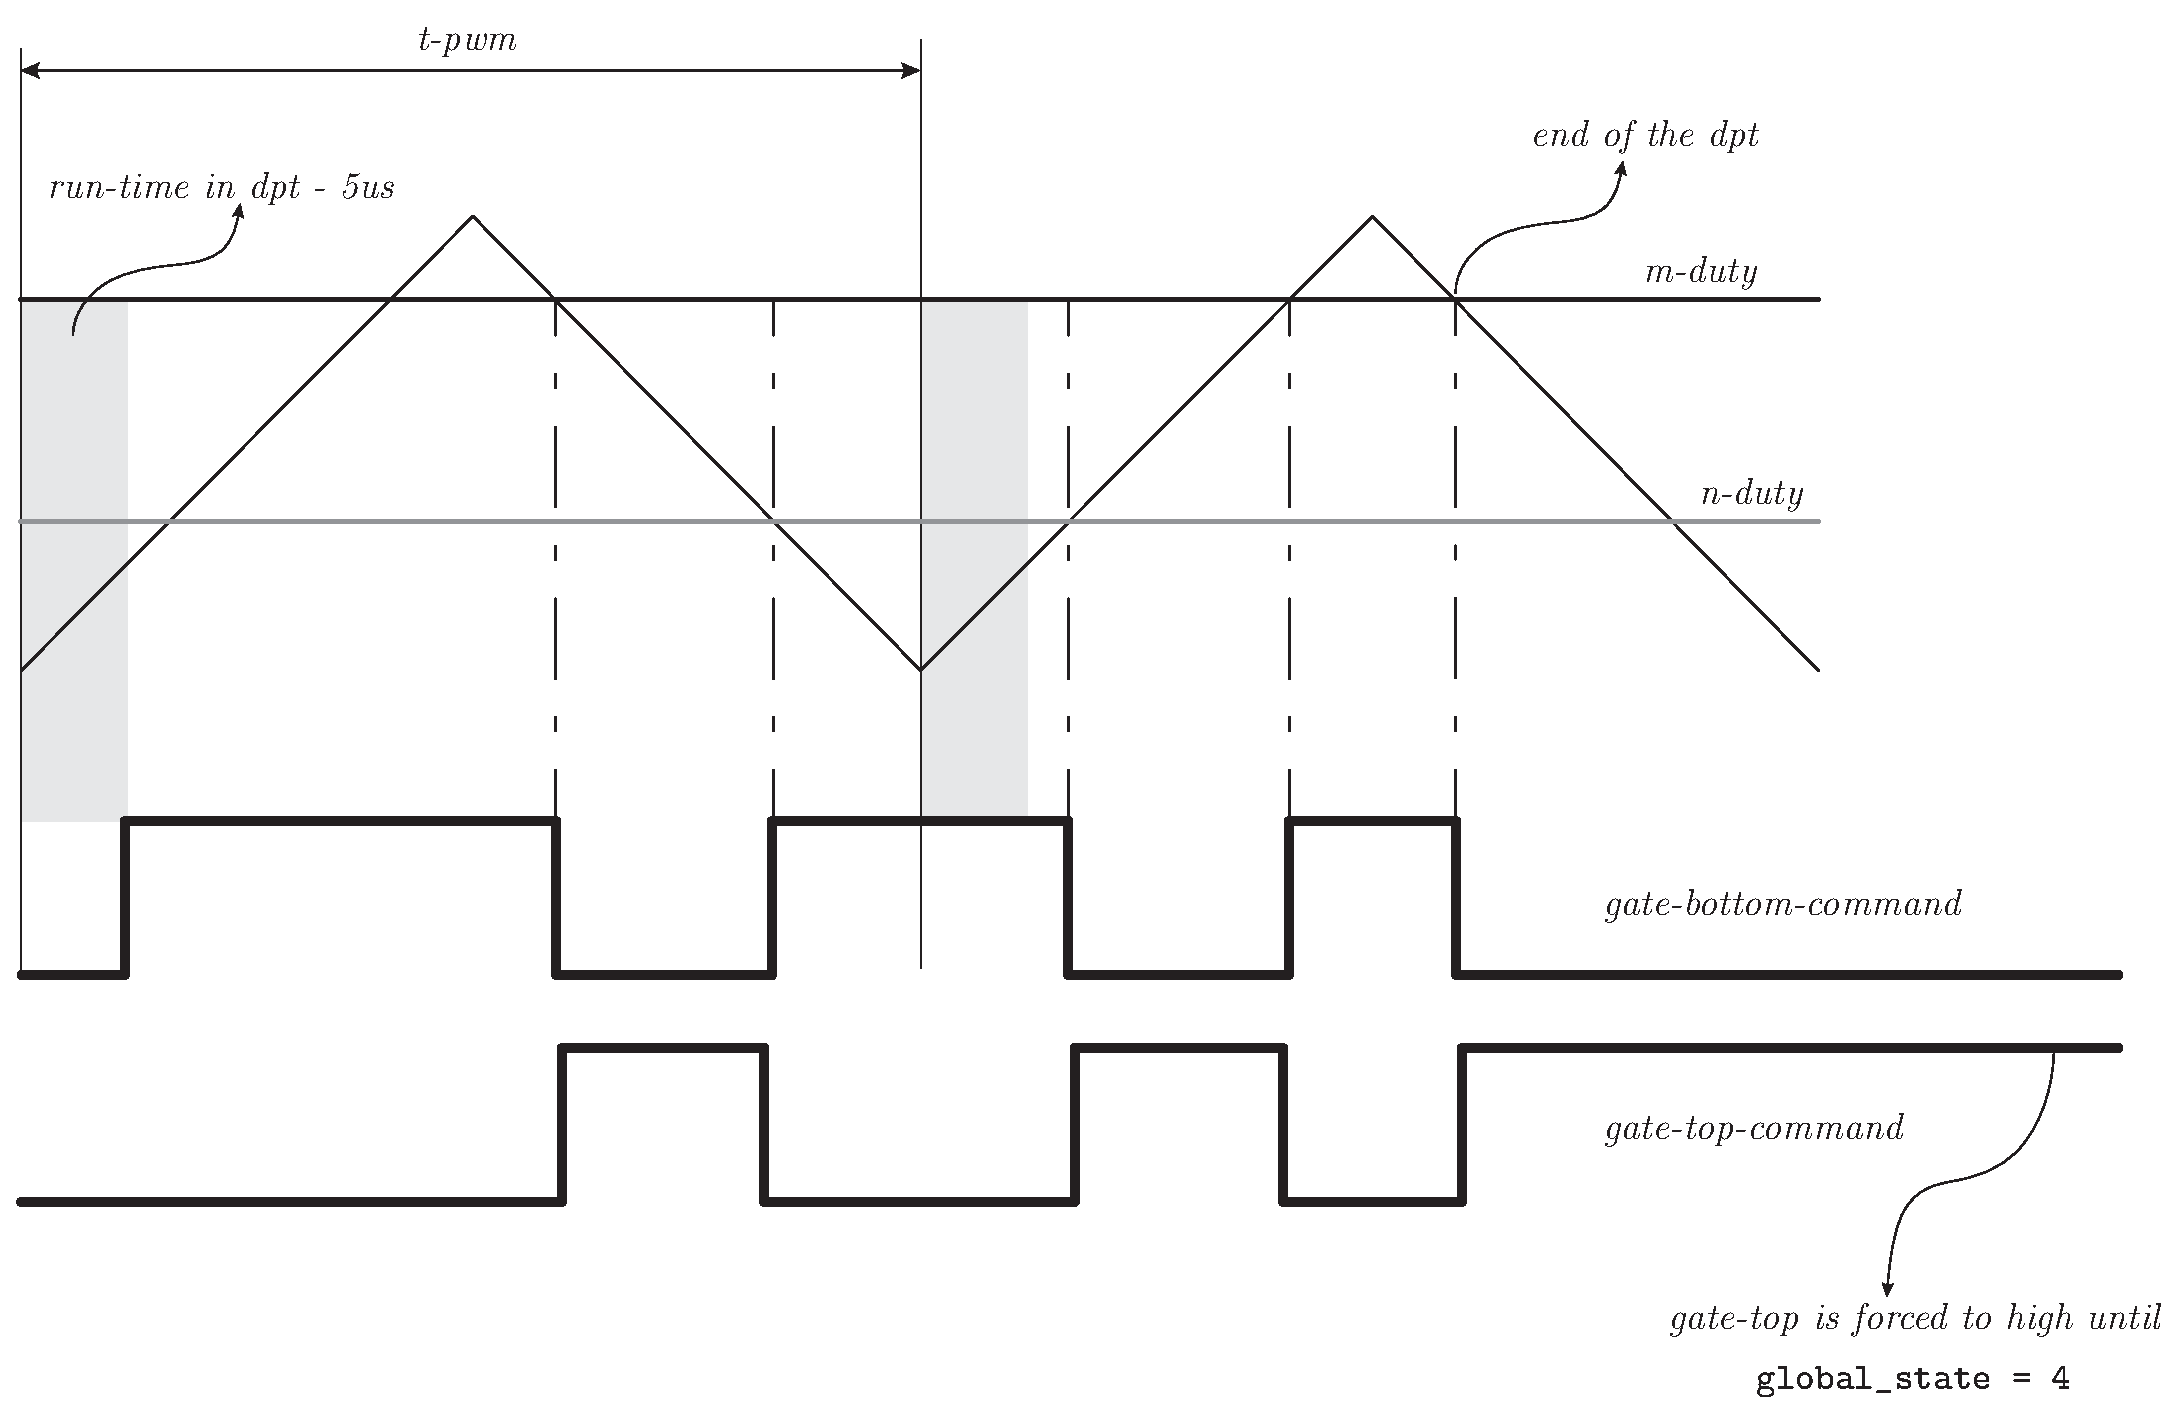
\includegraphics[width = 450pt, angle = 0, 
		keepaspectratio]{figures/double_pulse_test/dpt.eps}
		\captionsetup{width=0.5\textwidth, font=small}	
		\caption{Description how the double pulse is built.}
		\label{figure_1}
	\end{figure}
	
	\begin{figure}[H]
		\centering
		\begin{subfigure}{.5\textwidth}
			\centering
			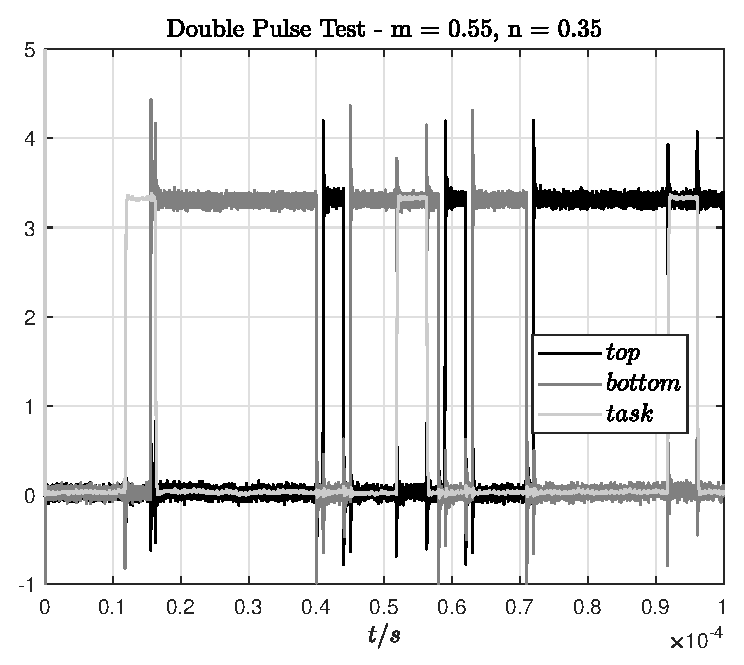
\includegraphics[width = 225pt, angle = 0, 
			keepaspectratio]{figures/double_pulse_test/measure_case_m055_n035.eps}
			\captionsetup{width=0.5\textwidth, font=small}	
			\caption{Double pulse test for the case $m = 0.55$ and $n = 0.35$.}
			\label{}
		\end{subfigure}%
		\begin{subfigure}{.5\textwidth}
			\centering
			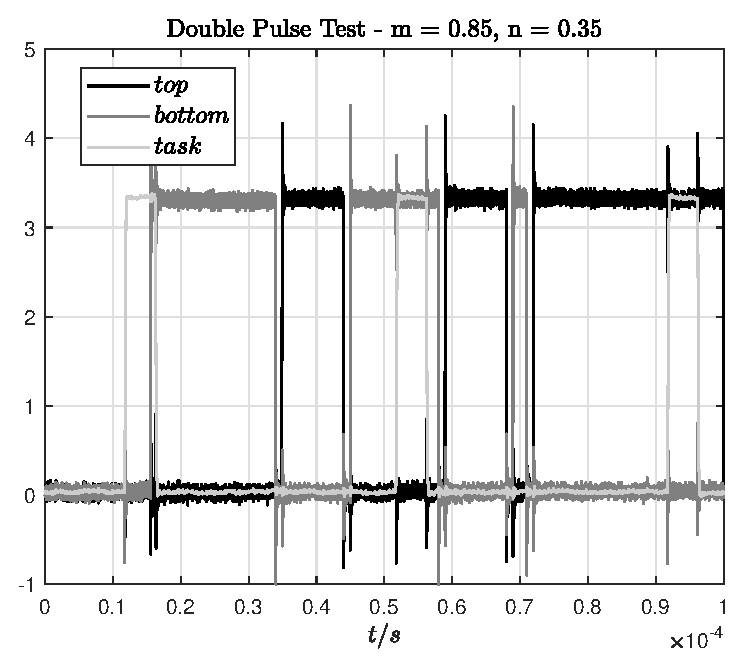
\includegraphics[width = 225pt, angle = 0, 
			keepaspectratio]{figures/double_pulse_test/measure_case_m085_n035.eps}
			\captionsetup{width=0.5\textwidth, font=small}	
			\caption{Double pulse test for the case $m = 0.85$ and $n = 0.35$.}
			\label{}
		\end{subfigure}
		\captionsetup{width=0.5\textwidth, font=small}
		\caption{Double pulse tests gate commands measure.}
		\label{}
	\end{figure}
	
	\begin{figure}[H]
		\centering
		\begin{subfigure}{.5\textwidth}
			\centering
			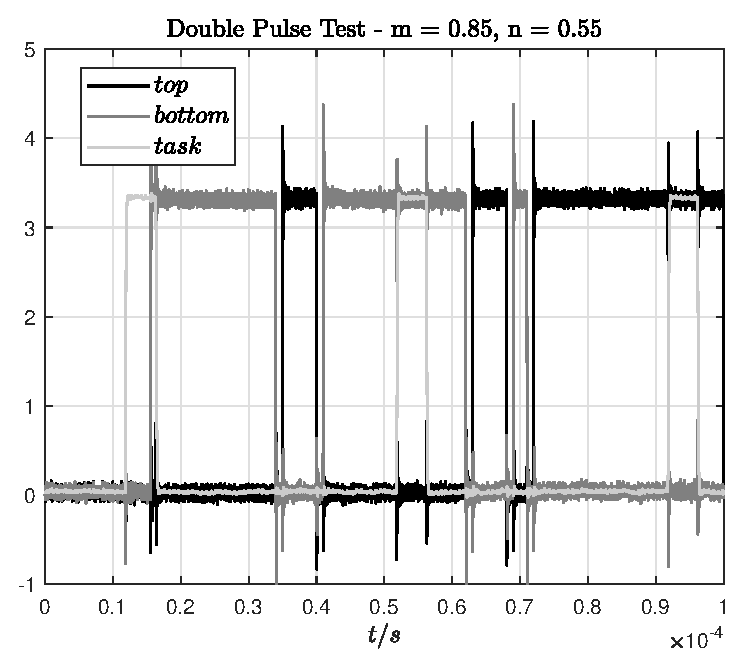
\includegraphics[width = 225pt, angle = 0, 
			keepaspectratio]{figures/double_pulse_test/measure_case_m085_n055.eps}
			\captionsetup{width=0.5\textwidth, font=small}	
			\caption{Double pulse test for the case $m = 0.85$ and $n = 0.55$.}
			\label{}
		\end{subfigure}%
		\begin{subfigure}{.5\textwidth}
			\centering
			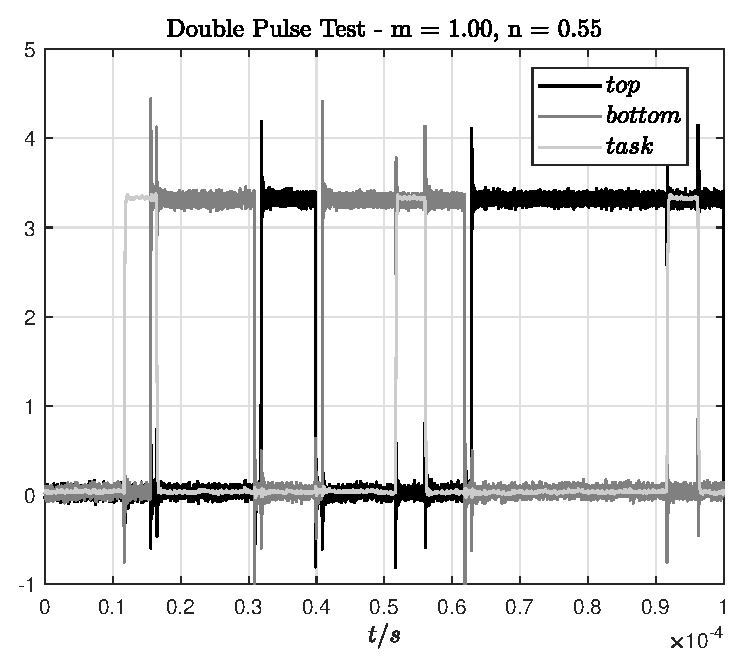
\includegraphics[width = 225pt, angle = 0, 
			keepaspectratio]{figures/double_pulse_test/measure_case_m100_n055.eps}
			\captionsetup{width=0.5\textwidth, font=small}	
			\caption{Double pulse test for the case $m = 1.00$ and $n = 0.55$.}
			\label{}
		\end{subfigure}
		\captionsetup{width=0.5\textwidth, font=small}
		\caption{Double pulse tests gate commands measure.}
		\label{}
	\end{figure} 
\end{example}

\section{List of Parameters}	

\begin{longtable}[l]{@{\extracolsep{\fill}}|p{16cm}|@{}}		
	\hline
	\rowcolor{gray!50}
	{\fontfamily{cmss}\selectfont \verb+param.inverter_current_max+} \\
	\hline 
	\endhead
	\hline
	\endlastfoot
	This parameter defines the maximum (readable) current of the inverter. It correlates the end-scale voltage of the ADC channel $u_{adc}^{max} = \SI{3.3}{\volt}$ with the end scale of the corresponding sensor in SI  $i_{inverter}^{max} = [\SI{}{\ampere}]$, which in this case will be end-scale of the current measure in Ampere. \\
\end{longtable}
\begin{longtable}[l]{@{\extracolsep{\fill}}|p{16cm}|@{}}		
	\hline
	\rowcolor{gray!50}
	{\fontfamily{cmss}\selectfont \verb+param.inverter_current_nom+} \\
	\hline
	\endhead
	\hline
	\endlastfoot
	This parameter defines the nominal current of the inverter. The nominal value is the value which is used for normalization. When the parameter ({\fontfamily{cmss}\selectfont \verb+param.inverter_current_u+}) results as 1, it corresponds to the nominal value.  \\
\end{longtable}
\begin{longtable}[l]{@{\extracolsep{\fill}}|p{16cm}|@{}}		
	\hline
	\rowcolor{gray!50}
	{\fontfamily{cmss}\selectfont \verb+param.inverter_current_scale+} \\
	\hline
	\endhead
	\hline
	\endlastfoot
	This parameter defines the conversion factor between the ADC channel measure (in \texttt{uint32\_t}) into the per unit float normalized current representation. This quantity is automatically calculated during initialization process.  \\
\end{longtable}
\begin{longtable}[l]{@{\extracolsep{\fill}}|p{16cm}|@{}}		
	\hline
	\rowcolor{gray!50}
	{\fontfamily{cmss}\selectfont \verb+param.inverter_current_u_offset+} \\
	\hline
	\endhead
	\hline
	\endlastfoot
	This parameter identifies the offset of the ADC channel (for bipolar signals). This variable is automatically generated during calibration process and used for the representation of the normalized current. \\
\end{longtable}
\begin{longtable}[l]{@{\extracolsep{\fill}}|p{16cm}|@{}}		
	\hline
	\rowcolor{gray!50}
	{\fontfamily{cmss}\selectfont \verb+param.inverter_current_v_offset+} \\
	\hline
	\endhead
	\hline
	\endlastfoot
	This parameter identifies the offset of the ADC channel (for bipolar signals). This variable is automatically generated during calibration process and used for the representation of the normalized current. \\
\end{longtable}
\begin{longtable}[l]{@{\extracolsep{\fill}}|p{16cm}|@{}}		
	\hline
	\rowcolor{gray!50}
	{\fontfamily{cmss}\selectfont \verb+param.inverter_current_w_offset+} \\
	\hline
	\endhead
	\hline
	\endlastfoot
	This parameter identifies the offset of the ADC channel (for bipolar signals). This variable is automatically generated during calibration process and used for the representation of the normalized current. \\
\end{longtable}

%	float iq_ref_fb;
%	float id_ref_fb;
%	
%	/* ADC measure and scaling
%	* *_max: this value identifies the end-scale of the sensor
%	* *_nom: this value identifies the nominal value used in the firmware
%	* *_scale: this value identifies the scaling from the integer of the ADC and the per unit used in the firmware
%	* *_offset: this value identifies the offset from the integer of the ADC and the per unit used in the firmware
%	*/
%	float temperature_igbt_inverter_max;		/* this value identifies the end-scale of the sensor */
%	float temperature_igbt_inverter_nom;		/* this value identifies the nominal value used in the firmware */
%	float temperature_igbt_inverter_scale;		/* this value identifies the scaling from the integer of the ADC and the per unit used in the firmware */
%	float temperature_igbt_inverter_offset;		/* this value identifies the offset from the integer of the ADC and the per unit used in the firmware */
%	
%	
%	float inverter_voltage_max;
%	float inverter_voltage_nom;
%	float inverter_voltage_scale;
%	float inverter_voltage_offset;
%	
%	float dclink_voltage_max;					/* this value identifies the end-scale of the sensor */
%	float dclink_voltage_nom;					/* this value identifies the nominal value used in the firmware */
%	float dclink_voltage_scale;					/* this value identifies the scaling from the integer of the ADC and the per unit used in the firmware */
%	float dclink_voltage_offset;				/* this value identifies the offset from the integer of the ADC and the per unit used in the firmware */
%	
%	float motor_voltage_max;
%	float motor_voltage_nom;					/* this variable is used for motor parameters normalization */
%	float motor_voltage_scale;
%	float motor_voltage_offset;
%	
%	float motor_current_max;
%	float motor_current_nom;					/* this variable is used for motor parameters normalization */
%	float motor_current_scale;
%	float motor_current_offset;
%	
%	float motor_torque_sign;					/* this variable is used to change the sign of the torque reference generated by the speed loop */
%	
%	/* ADC variables */
%	float inverter_current_u;
%	float inverter_current_v;
%	float inverter_current_w;
%	float dclink_voltage;
%	float temperature_igbt_inverter_u;
%	float temperature_igbt_inverter_v;
%	float temperature_igbt_inverter_w;
%	float temperature_ambient;
%	float temperature_heatsink;
%	float temperature_motor;
%	
%	/* PWM period: it corresponds to the period of the main control process */
%	float inverter_t_pwm;
%	float base_freq_inv;
%	
%	/* variables used into the control algorithms */
%	float inverter_theta_hat_sin;
%	float inverter_theta_hat_cos;
%	float inverter_current_d;
%	float inverter_current_q;
%	float inverter_current_alpha;
%	float inverter_current_beta;
%	float torque_lim_top;
%	float torque_lim_bottom;
%	float omega_ref_pu;
%	float omega_hat;
%	float omega_hat_pu;
%	float theta_hat;
%	float torque_hat;
%	float torque_ref;
%	float cos_theta;
%	float sin_theta;
%	float dclink_voltage_compensation;
%	float dclink_voltage_flt;
%	float u_out_lim;
%	
%	/* speed control PI gains */
%	float kp_omega;
%	float ki_omega;
%	
%	/* currents control PI gains */
%	float kp_inv_id;
%	float ki_inv_id;
%	float kp_inv_iq;
%	float ki_inv_iq;
%	
%	/* state observer gains */
%	float bemf_obsv_kalman_omega;
%	float bemf_obsv_kalman_theta;
%	float bemf_obsv_fb_p;
%	float bemf_obsv_p;
%	
%	/* variables used as references */
%	float inverter_current_reference_q;
%	float inverter_current_reference_d;
%	float id_ext_ref;
%	float iq_ext_ref;
%	
%	/* variables used as fault thresholds */
%	float inverter_overcurrent_fault_th;
%	float inverter_overtemperature_fault_th;
%	float dclink_overvoltage_fault_th;
%	float dclink_undervoltage_fault_th;
%	float omega_max_th;
%	
%	/* variables used for normalization of the PMSM motor */
%	float motorc_omega_bez;
%	float motorc_m_scale;
%	float motorc_rs_norm;
%	float motorc_ls_norm;
%	float motorc_ld_norm;
%	float motorc_lq_norm;
%	float motorc_phi_m_norm;
%	float motorc_xbez;
%	float motorc_lbez;
%	
%	/* mirrors of the global state machine variables */
%	uint8_t 	global_state;
%	uint32_t 	global_fault_state_description;
%	uint8_t 	global_cmd;
%	
%	/* mirrors of the inverter state machine variables */
%	uint8_t 	inverter_ctrl_state;
%	uint8_t 	inverter_ctrl_mode;
%	uint32_t 	inverter_fault_state_description;
%	uint8_t 	inverter_cmd;
%	
%	/* mirrors of the global command word generation state */
%	uint8_t 	global_cmd_word_generation_state;
%	
%	/* mirrors of the pwm status variables */
%	uint8_t 	pwm_enable;
%	
%	/* mirrors of the brake status variables */
%	uint8_t 	brake_enable;
%	
%	/* variables used for the signal generator */
%	float signal_generator_freq_bez; 			/* base frequency */
%	float signal_generator_u_ref_out;			/* amplitude of the output signal in Volt */
%	float signal_generator_i_ref_out;			/* amplitude of the output signal in Ampere */
%	float signal_generator_output;				/* signal generator output */
%	
%	/* variables used into CAN BUS */
%	float duty_reference;				/* thrust input command */
%	float duty_reference_flt;			/* filtered thrust input command */
%	float reference_flt_fcut;			/* filtered thrust input command: filter frequency cut */
%	
%	uint32_t debug_mode;
%	uint32_t mu;
%	uint32_t mv;
%	uint32_t mw;
%	
%	float double_pulse_m_duty;
%	float double_pulse_n_duty;
%	uint8_t double_pulse_leg;
%	uint32_t double_pulse_test_counter;



\clearpage
\begin{thebibliography}{99}
	\bibitem{staffler} 
	M. Schroedl, M. Hofer, W. Staffler, \emph{Combining INFORM method, voltage model and mechanical observer for sensorless control of PM synchronous motors in the whole speed range including standstill}. Springer 2006.
	
	\bibitem{rodriguez} 
	J. Rodriguez, P. Cortes, \emph{Predictive Control of Power Converters and Electrical Drives}. Wiley 2012.
	
	\bibitem{krause} 
	P. Krause, O. Wasynczuk, S. Sudhoff, S. Pekarek, \emph{Analysis of Electric Machinery and Drive Systems}. Third Edition Wiley 2013.
	
	\bibitem{bianchi} 
	N. Bianchi, T. Jahns,  \emph{Design, analysis, and control of interior PM synchronous machines}. CLEUP 2004.
	
	\bibitem{plet1} 
	G. L. Plett,  \emph{Battery Modeling. Volume I}. Artech House 2015.
	
	\bibitem{plet2} 
	G. L. Plett,  \emph{Battery Modeling. Volume II}. Artech House 2015.
	
	\bibitem{plet_p1} 
	G. L. Plett,  \emph{Extended Kalman filtering for battery management systems of LiPB/based HEV battery packs. Part 1. Background}. Journal of Power Sources 134 (2004).
	
	\bibitem{plet_p2} 
	G. L. Plett,  \emph{Extended Kalman filtering for battery management systems of LiPB/based HEV battery packs. Part 2. Modeling and identification}. Journal of Power Sources 134 (2004).	
	
	\bibitem{plet_p3} 
	G. L. Plett,  \emph{Extended Kalman filtering for battery management systems of LiPB/based HEV battery packs. Part 3. State and parameter estimation}. Journal of Power Sources 134 (2004)	
	
\end{thebibliography}
%\end{onehalfspace}
\end{document} 